%%%% HELP
%%% 


\documentclass{swfcthesis}
\usepackage{makecell}
\usepackage[export]{adjustbox}
\usepackage{lipsum}
\usepackage{mwe}


\renewcommand{\acknowledgmentspage}{% Acknowledgments page  
  \phantomsection%
  \addcontentsline{toc}{chapter}{Acknowledgments}
  \chapter*{Acknowledgments}

  I would like to thank my supervisor Mr. WANG Xiaolin for his continuous support of my
  four years undergraduate study. I am extremly thankful to him for sharing expertise, and
  sincere and valuable guidance and encouragement extended to me.
    
  What I most want to thank is my girlfriend. She tolerated me when I finished this
  graduation project many nights did not accompany her, gave me support, encouraged me,
  and did not complain. So I would like to name this simple operating system as RongOS. Rong
  is the last word of her name. Thank you, my dearest.
  
  My special thanks to a great company - Google, I think I need to thank you in this very
  formal place in my graduation thesis. Every time you gave me a lot of help, the
  knowledge and other abilities I learned from you will have a profound impact on my
  future life. I am grateful for every search, because I know you will give me the results
  I want. Without you, this paper cannot be completed. Thank you.
    
}

\renewcommand{\advisorinfopage}{% Advisor info page
  \phantomsection%
  \addcontentsline{toc}{chapter}{Supervisor}
  \chapter*{Supervisor}
  Xiaolin WANG (Mr.), 49 years old, got his MSc degree at University of Greenwich in
  UK\@. Currently he's been working as a lecturer at the School of Big Data and
  Intelligence Engineering, Southwest Forestry University in China, teaching Linux,
  Operating Systems, and Computer Networking.
  \clearpage}

\renewcommand{\contentsname}{Contents}
\renewcommand{\listfigurename}{List of Figures}
\renewcommand{\listtablename}{List of Tables}
\renewcommand{\figurename}{Fig.}
\renewcommand{\tablename}{Table}
\renewcommand{\listingscaption}{Code} % used by minted
\renewcommand{\listoflistingscaption}{List of Codes}

\addbibresource{thesis.bib}

\begin{document}

\Title{RongOS --- 一个简单操作系统的设计与实现}
\Author{蒲启元}
\Advisor{王晓林}
\AdvisorTitle{讲师}
\Month{六}
\Year{二〇一八}

\Subject{计算机科学与技术专业} %专业名称(比如 电子信息工程专业)

\Abstract{操作系统管理着计算机的硬件和软件资源,它是向上层应用软件提供服务(接口)的核心系
  统软件,这些服务包括进程管理,内存管理,文件系统,网络通信,安全机制等。操作系统的设计与
  实现则是软件工业的基础。为此,在国务院提出的《中国制造2025》中专门强调了操作系统的开
  发\cite{china_2025}。但长期以来,操作系统核心开发技术都掌握在外国人手中,技术受制,对于我
  们的软件工业来说很不利。本项目从零开始设计开发一个简单的操作系统,包括boot loader,中断,
  内存管理,图形接口,多任务等功能模块,以及能运行在这个系统之上的几个小应用程序。尽管这
  个系统很简单,但它是自主开发操作系统的一次尝试。}

\Keywords{操作系统,进程,内存,中断,boot loader}

\enTitle{RongOS --- A simple OS implementation}

\enAuthor{Qiyuan PU}

\enAbstract{Operating system manages the hardware and software resources in a running
  computer system. It is the core of any modern software system and provides services
  (interfaces) to upper layer applications. The services it provides include process
  management, memory management, file system, network communication, security mechanism
  and more. Operating system development is the foundation and core of software
  industry. Therefore, \emph{Made in China 2025} emphasizes the development of operating
  system that put forward by The State Council of China. For long time, however, the OS
  kernel development technology is dominated by foreigners. This technical limitation is
  detrimental to the development of our software industry. In this project, we presents a
  simple operating system which includes a boot loader, interrupt services, memory
  management functions, a graphic interface, and multi-process management functions. Also,
  some trivial user-level applications are provided for system testing purpose. This
  simple toy OS is an experimental trial for developing an operating system from scratch.}

\enKeywords{operating system, boot loader, interrupt, process management, memory management}

%%% 下面六行不要动!
\makepreliminarypages% 封面
\frontmatter          
\tableofcontents     % 目录
\listoffigures       % 插图目录
\listoftables        % 表格目录
\listoffixmes{}

\mainmatter{}

\chapter{Introduction}
This section will introduce the purpose and current status of the operating system
research. The setup of the development environment will also be presented here.


\section{Background}

Contemporary software systems are beset by problems that create challenges and
opportunities for broad new OS research. There are five areas could improve user
experience including dependability, security, system configuration, system extension, and
multiprocessor programming.

The products of forty years of OS research are sitting in everyone's desktop computer,
cell phone, car, etc., and it is not a pretty picture.  Modern software systems are
broadly speaking complex, insecure, unpredictable, prone to failure, hard to use, and
difficult to maintain. Part of the difficult is that good software is hard to write, but
in the past decade, this problem and more specific shortcomings in systems have been
greatly exacerbated by increased networking and embedded systems, which placed new demands
that existing architectures struggled to meet. These problems will not have simple
solutions, but the changes must be pervasive, starting at the bottom of the software
stack, in the operating system.

The world needs broad operating system research. Dependability, security, system
configuration, system extension, and multi-processor programming illustrate areas were
contemporary operating systems have failed to meet the software challenges of the modern
computing environment\cite{hunt2005broad}.


\section{Preliminary Works}

\subsection{Development Environment}

\begin{description}
\item[OS platform:] Debian 9, Linux kernel 4.12.0-1-amd64
\item[Editor:] GNU Emacs 25.2.2
\item[Run time VM:] QEMU emulator 2.8.1
\item[Assembler:] Nask
\item[Compiler:] CC1(Based on gcc)
\item[Debugger:] GNU gdb 7.12
\item[Version Control:] git 2.15
\end{description}

\subsection{Tools}

Some tools were used to develop RongOS, See \emph{tools}\footnote{\url{https://github.com/Puqiyuan/RongOS/tree/master/z_tools}}. Note that
these tools are Windows executable. Please install wine if you want to run these tools on
Linux. In these tools, the most important ones are:

\begin{description}
\item[nask.exe:] the assembler, a modified version of NASM\cite{30_os}
\item[cc1:] the C compiler
\end{description}

\subsection{Platform Setup}

The development platform (mainly the Debian system) was set up by following the
\emph{Debian Installation
  tutorial}\footnote{\url{http://cs2.swfc.edu.cn/~wx672/lecture_notes/linux/install.html}}. The
main steps include:
\begin{enumerate}
\item Installing the base Debian system;
\item Installing necessary software tools, such as emacs, web browser, qemu, wine, etc.;
\item Cloning configuration files by following the tutorial mentioned above;
\item Some more fine tweaks to satisfy my personal needs.
\end{enumerate}

\subsubsection{Qemu}

QEMU is a generic and open source machine emulator and virtualizer\cite{wiki:qemu}. In
this project, QEMU was used as the test bed.

Installing QEMU for my x86\_64 architecture can be easily done by executing the following
command:
\begin{verbatim}
     $ sudo apt-get install qemu-system-x86_64
\end{verbatim}

\subsubsection{Wine}

Wine (originally an acronym for ``Wine Is Not an Emulator'') is a compatibility layer
capable of running Windows applications on several POSIX-compliant operating systems, such
as Linux, macOS, and BSD\cite{wiki:wine}.

Because the tools I used in this project are in Windows executable format, so on Debian system,
Wine is needed to be installed:

\begin{verbatim}
     $ sudo apt-get update
     $ sudo apt-get install wine
\end{verbatim}

\subsubsection{Debian i386 support}

On 64-bit systems you need to enable multi-arch support for running 32-bit Windows
applications (many modern apps are still 32-bit, also for large parts of the Windows
subsystem itself). Our development tools were 32-bit Windows applications, so we needed to
have i386 support for our 64-bit Linux system.

\begin{verbatim}
     $ sudo dpkg --add-architecture i386
     $ sudo apt-get update
\end{verbatim}

\iffalse %%%%%%%%%%%%%%%%%%%%%%%%%%%%%%%%%%%%%%%%%%%%%%%%%%%%%%%%%%%%%%%%%%%%%%%%%%%%%%%%%%%%%%%%%
%\chapter{Leading Knowledge}
%\label{cha:leading-knowledge-1}

%\section{Layers}
%\label{sec:layers}

%\section{Memory Management}
%\label{sec:memory-management}

%\subsection{Overview}
%\label{sec:overview}

%\subsection{Round Down/Up and Page Size}
%\label{sec:round-downup-page}


%\section{Mouse}
%\label{sec:mouse}

%\section{The Leap --- Road to the 32 Bit Mode}
%\label{sec:leap-road-32}

%\section{Data Structure}
%\label{sec:data-structure}

%\section{Programmable Interrupt Controller}

\section{C Language Basic}

\section{Segments and Descriptors}
The so-called segmentation is to divide a total of 4 GB of memory into many blocks in its
own way. The start address of each block is treated as 0.

In this way, in order to represent a segment, the following information is required:
\begin{itemize}
\item The size of the segment
\item Where is the starting address of the segment
\item Segment management properties
\end{itemize}

All this information is represented by 8 bytes(64 bits). But the register used to specify
the segment is only 16 bits. Therefore, the segment selector is stored in the segment
register, and the segment management information(the above three information) is
referenced by the segment selector. Although the segment register has 16 bits, only high 13
bits are available due to the CPU design. Therefore, the segment selector is in the range
of 0 to 8191. In total, there are 8192 segments, and a total of 8192 × 8 = 65536(64KB) bytes are
required to store the management information of these segments. This 64-byte message is
called GDT. Obviously, the CPU does not have such a large storage capacity. So store this
information somewhere in memory. A special register in the CPU is GDTR(global descriptor
table register). This register is used to reference the GDT address in memory and record
how many valid segments are set.



\section{Instruction Set}

An instruction set architecture (ISA) is an abstract model of a computer. It is also
referred to as architecture or computer architecture. An ISA defines everything a machine
language programmer needs to know in order to program a computer.

An ISA may be classified in a number of different ways. A common classification is by
architectural complexity. A complex instruction set computer (CISC) has many specialized
instructions, some of which may only be rarely used in practical programs. A reduced
instruction set computer (RISC) simplifies the processor by efficiently implementing only
the instructions that are frequently used in programs, while the less common operations
are implemented as subroutines, having their resulting additional processor execution time
offset by infrequent use.

On traditional architectures, an instruction includes an opcode that specifies the
operation to perform, such as add contents of memory to register—and zero or more operand
specifiers, which may specify registers, memory locations, or literal data\cite{wiki:isa}.

This simple RongOS is based on x86 architecture, the following instructions are commonly
used in programming RongOS:%

\begin{description}
\item[db:] the abbreviation of define byte, write a byte, also 8 bits to file.
\item[resb:] the abbreviation of reserve byte, reserved bytes and filling \emph{0x00} in these reserved space.
\item[dw:] the abbreviation of define word, write two bytes, also 16 bits to file.
\item[dd:] the abbreviation of define double-word, write four bytes, also 32 bits to file.
\item[org:] load the program to specified address.
\item[jmp:] jump to another instruction.
\item[mov:] assign the right value to left variable.
\item[jc:] the abbreviation of jump if carry, it means if carry flag is 1, jump.
\item[jnc:] jump if not carry.
\item[jae:] jump if above or equal.
\item[jbe:] jump if below or equal.
\item[jb:] jump if below.
\item[equ:] equ is the abbreviation of equal.
\item[ret:] end of function, return.
\item[in:] get signal from device.
\item[out:] send signal to device.
\item[cli:] clear interrupt flag, set it to 0.
\item[sti:] set interrupt flag, set it to 1.
\item[pushfd:] push flags double-word.
\item[popfd:] pop flags double-word.
\item[lgdt:] load content from specified memory to initialize GDT (global descriptor table)
  register.
\item[lidt:] load content from specified memory to initialize IDT (interrupt descriptor
  table) register.
\end{description}

\section{x86 Registers}

In computer architecture, a processor register is a quick accessible location available
to a computer's central processing unit (CPU). Registers usually consist of a small amount
of fast storage, although some registers have specific hardware functions, and may be
read-only or write-only.  Almost all computers, whether load/store architecture or not,
load data from a larger memory into registers where it is used for arithmetic operations
and is manipulated or tested by machine instructions. Manipulated data is then often
stored back to main memory, either by the same instruction or by a subsequent one. Modern
processors use either static or dynamic RAM as main memory, with the latter usually
accessed via one or more cache levels\cite{wiki:registers}.

Processor registers are normally at the top of the memory hierarchy, and provide the
fastest way to access data. The term normally refers only to the group of registers that
are directly encoded as part of an instruction, as defined by the instruction
set. Registers are normally measured by the number of bits they can hold, for example, an
``8-bit register'' or a ``32-bit register''. For x86 architecture, the following registers
exist, see 3.4.1 and 3.4.2 \cite{guide2011intel}:

\begin{multicols}{3}
  \begin{description}
  \item[ax:] accumulator
  \item[bx:] base
  \item[cx:] counter
  \item[dx:] data
  \item[bl:] base low
  \item[al:] accumulator low
  \item[cl:] counter low
  \item[dl:] data low
  \item[bh:] base high
  \item[ah:] accumulator high
  \item[ch:] counter high
  \item[dh:] data high
  \item[sp:] stack pointer
  \item[bp:] base pointer
  \item[si:] source index
  \item[di:] destination index
  \item[es:] extra segment
  \item[cs:] code segment
  \item[ss:] stack segment
  \item[ds:] data segment
  \item[fs:] no name
  \item[gs:] no name
  \end{description}
\end{multicols}

Among these registers, \emph{bx, bp, si} and \emph{di} can be used to specify the
address of memory. But \emph{ax, cx, dx} and \emph{sp} can not. When \emph{mov}
instruction is used, the number of bits of source number should be the same with
destination operand.

\begin{description}
\item[16-bit registers:] \emph{ax, cx, dx, bx, sp, bp, si, di, es, cs, ss, ds}, and \emph{fs}.
\item[8-bit registers] \emph{al, cl, dl, bl, ah, ch, dh}, and \emph{bh}.
\end{description}
Actually, as shown in Fig.~\ref{fig:regs}, all these 8-bit registers are parts of
corresponding 16-bit registers.

\begin{figure}[!htbp]
  \centering
  \begin{center}
    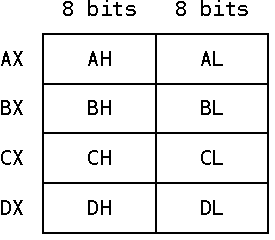
\includegraphics[width=.4\textwidth]{registers}
  \end{center}
  \caption{x86 registers}
  \label{fig:regs}
\end{figure}

\section{Interrupt Call}

BIOS interrupt calls perform hardware control or I/O functions requested by a program,
return system information to the program, or do both. A key element of the purpose of BIOS
calls is abstraction. The BIOS calls perform generally defined functions, and the specific
details of how those functions are executed on the particular hardware of the system are
encapsulated in the BIOS and hidden from the program\cite{wiki:bios-int}. The interrupt
calls are commonly used in RongOS are listed in Table~\ref{tbl:intcall}.

\begin{table}[!ht]
  \centering\tabulinesep=2mm
  \begin{tabu}{X[l,m,-1]X[l,m]X[-1,l,m]X[-1,l,m]}
    \tabucline-\rowfont\bfseries
    Interrupt\par{}Number & Register Parameter & Return Value & Function\\ \tabucline-
    0x10 &
    ah=0x0e(write character in tty mode)\par{}
    al=character code\par{}
    bh=0, bl=colorcolor& null & video services \\\tabucline-
    0x13 &
    ah=0x02(read sectors)\par{}
    ah=0x03(write sectors)\par{}
    ah=0x04(verify sectors)\par{}
    ah=0x0c(seek to specified track)\par{}
    al=number of sectors processing\par{}
    ch=cylinder \& 0xff  cl=sector number\par{}
    dh=header number dl=driver number\par{}
    es:bx=buffer address &
    FLACS.CF=0\par{}
    no error, ah = 0\par{}
    FLAGS.CF=1\par{}
    error, ah=error number\par{}& disk services \\ \tabucline-
  \end{tabu}
  \caption{RongOS interrupt calls}\label{tbl:intcall}
\end{table}

\section{Memory Map}

In the boot process, a memory map is passed on from the firmware in order to instruct an
operating system kernel about memory layout. It contains the information regarding the
size of total memory, any reserved regions and may also provide other details specific to
the
architecture\footnote{http://hypervsir.blogspot.com/2014/09/approach-to-retrieving-bios-memory-map.html}. For
loading RongOS to memory, the memory layout should be clarified as in
Table~\ref{tbl:memlayout}.


\begin{table}[!ht]
  \centering\tabulinesep=2mm
  \begin{tabu}{%
      >{\texttt\bgroup}r<{\egroup}@{\,--\,}>{\texttt\bgroup}l<{\egroup}%
      >{\texttt\bgroup}r<{\egroup}@{\,--\,}>{\texttt\bgroup}l<{\egroup}%
      >{\texttt\bgroup}l<{\egroup}l}%
    \tabucline-\rowfont\bfseries%
    \multicolumn{2}{l}{Range (in hexadecimal)} &%
    \multicolumn{2}{l}{Range (in decimal)} &%
    \multicolumn{1}{l}{Size (in bytes)} & Usage \\ \tabucline-
    0000 & 03ff & 0000 & 1023 & 1024 &  interrupt vector table \\ 
    0400 & 04ff & 1024 & 1279 & 256 & BIOS data area \\ 
    0500 & 051f & 1280 & 1311 & 32 & Reserved \\ 
    0520 & 7bff & 1312 & 31743 & 30432 & conventional memory \\ 
    7c00 & 7dff & 31744 & 32255 & 512 & master boot record \\ 
    7e00 & 9ffff & 32256 & 655359 & 623104 & conventional memory \\ 
    a0000 & affff & 655360 & 720895 & 64K & VGA graphics RAM \\ 
    b0000 & b7fff & 720896 & 753663 & 32K & monochrome text mode \\ 
    b8000 & bffff & 753664 & 786431 & 32K & color text mode \\ 
    c0000 & c7fff & 786432 & 819199 & 32K & VGA video ROM \\ 
    c8000 & cbfff & 819200 & 835583 & 16K & IDE hard drive \\ 
    cc000 & cffff & 835584 & 851967 & 16K & optional adapter \\ \tabucline-
  \end{tabu}
  \caption{RongOS Memory Layout}\label{tbl:memlayout}
\end{table}

\section{Floppy Disk}

There are many ways to boot an operating system, from hard disk, USB, floppy disk, etc.
The structure of floppy disk is simple and for this simple operating system it's enough.

Fig.~\ref{fig:flpy1.png} shows the inside of a floppy disk:
\begin{figure}[!ht]
  \centering
  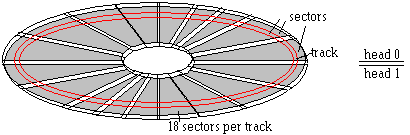
\includegraphics[width=.5\textwidth]{../figs/bootLoader/flpy1.png}
  \caption{Floppy disk structure}
  \label{fig:flpy1.png}
\end{figure}

A floppy disk, also called a floppy, diskette, or just disk, is a type of disk storage
composed of a disk of thin and flexible magnetic storage medium, sealed in a rectangular
plastic enclosure lined with fabric that removes dust particles. Floppy disks are read and
written by a floppy disk drive (FDD)\cite{wiki:floppy}.

For 3.5 inch HD floppy,  There are 80 cylinders from the outermost to
the core on each side, numbering 0, 1, \ldots, 79. The head can assign be 0 or 1,
representing two sides of floppy. When specify head number and cylinder number, forming a
ring, named track in jargon. The track is large so we divide it to 18 small parts, named
sector. A sector can store 512 byte. So the capacity of a floppy is:

\[18 \times 80 \times 2 \times 512 = 1474560\,Byte = 1440\,KiB\]

\fi %%%%%%%%%%%%%%%%%%%%%%%%%%%%%%%%%%%%%%%%%%%%%%%%%%%%%%%%%%%%%%%%%%%%%%%%%%%%%%%%%%%%%%%%%%%%%%%%


\chapter{Design}

This chapter describes the design issues in the entire software system, including system startup,
the kernel, APIs, and some applications.


\section{Top Level Design}

As shown in Fig.~\ref{fig:top-level} shown, \fxerror{correct picture}, all applications
require services from the
operating system through a set of function calls. This set of functions provided by the OS
kernel is usually called \emph{system calls}. However, the user applications do not invoke
these system calls directly. Instead, they call the API library functions. The process in
which the API invokes a system call and hands over processing to the kernel is called
\emph{trapping}.

Within the kernel, there are some important software modules working to keep the system
running well. The process control subsystem provides graphics processing, CPU scheduling,
and memory management functions for processes. \fxerror{do you have VFS?} The file
subsystem provides a friendly way to the user processes for accessing disk data. For
example, to launch an application program stored on the disk, the function in the file
system must be invoked to find the specific application. All of these subsystems may
interact with the driver or hardware control module so as to operate on the system
hardwares.

\begin{figure}%[!htbp]
  \centering
  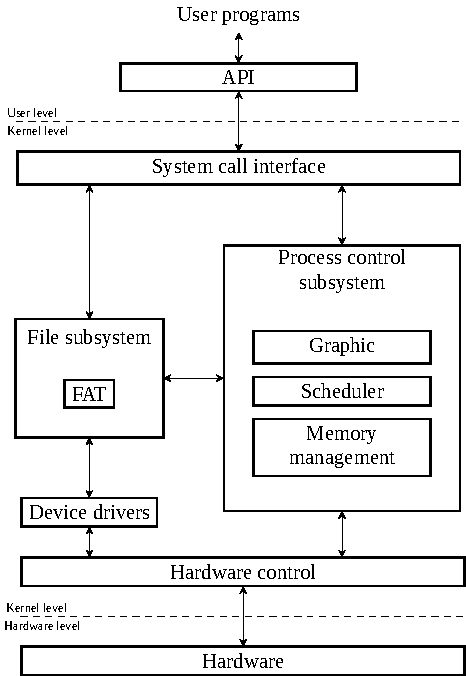
\includegraphics[width=.7\textwidth]{kernel-block.pdf}
  \caption{Top-level design}
  \label{fig:top-level}
\end{figure}


\section{Detailed Design}
\label{sec:detailed-design}

This section discusses the system design in details, including the function of each
module, data structures used in boot loader, kernel, API, and APPs.

\subsection{Boot Up}
\label{sec:boot-up}

At this stage the boot loader loads the operating system kernel into memory. This is done
in the following four steps:
\begin{enumerate}
\item Display boot information;
\item Read the second sector;
\item Read two sides of a track;
\item Read the next cylinder until all twenty cylinders have been read.
\end{enumerate}

At this stage, it is also necessary to complete the 32-bit protection mode switch and jump
to the entry point of the operating system.

\subsection{Kernel}
\label{sec:kernel}

The kernel receives the API calls from user processes, and operates the
hardwares through the device drivers.\fxerror{say some more.}

\subsubsection{Memory Management}
\label{sec:memory-management-1}

Memory management refers to the technology that allocates and uses computer memory
resources while the software is running. Its main purpose is how to allocate efficiently
and quickly, and release for reusing memory resources when appropriate. This is critical
to any advanced computer system where more than a single process might be underway at any
time.

Several methods have been invented to improve the effectiveness of memory management. For
modern operating systems, memory virtualization technology is used. This technique
separates the memory space used by the process from the actual physical memory. Processes
that are temporarily not running will be moved to secondary storage through paging or
swapping. How virtual memory is designed and how it is implemented will have a wide impact
on the overall system performance.

For RongOS, table ~\ref{tab:memo-tab} reflects the memory management system.
\begin{table}[!ht]
  \centering
  \begin{tabular}{|c|c|}
    \hline
    Start Address & Free Size \\
    \hline
    1 & 301 \\
    \hline
    348 & 50 \\
    \hline
    800 & 1000 \\
    \hline
    3001 & ... \\
    \hline
  \end{tabular}
  \caption{memory management table}
  \label{tab:memo-tab}
\end{table}
An \emph{entry} is a record reflects how much memory space is free from where. Actually,
this table is an member \emph{struct FREEINFO} in \emph{struct MEMMAN}.




\paragraph{Data Structures used in MM}

\begin{codeblock}[1]
\begin{ccode}
struct FREEINFO
{ 
  unsigned int addr; /* start address of free space */
  unsigned int size; /* size of free mem in bytes*/
};
\end{ccode}
\end{codeblock}
\begin{itemize}
\item % (Code~\ref{src:FREEINFO})
  is used to record the size in bytes of free memory while
  the system is running.
\end{itemize}

\begin{codeblock}[1]
\begin{ccode}
struct MEMMAN
{ 
  int frees;    /* free memory blocks */
  int maxfrees; 
  int lostsize; /* the sum of the failed memory size to freed*/
  int losts;    /* number of failures */
  struct FREEINFO free[MEMMAN_FREES]; /* free memory block info */
};
\end{ccode}
\end{codeblock}
\begin{itemize}
\item is used to record the entire
  memory usage, such as the total remaining free memory space and \emph{entry}.
\end{itemize}

\paragraph{Memory Management Functions}
\csingle|unsigned int memtest(unsigned int start, unsigned int end);|
\begin{itemize}
\item Check the memory capacity and confirm that the memory is intact. \emph{start} is the start
  address of the memory check and \emph{end} is the end address of the memory
  check. This function returns the maximum value of available addresses. Memory is
  available between this value and the \emph{start} value.
\end{itemize}


\csingle|unsigned int memman_total(struct MEMMAN* man);|
\begin{itemize}
\item Report the sum of all empty space. It will look for each \emph{entry} in the
  \emph{man} to add up the free space in it.
  
\end{itemize}

\csingle|unsigned int memman_alloc(struct MEMMAN *man, unsigned int size);|
\begin{itemize}
\item Allocate memory to the application, where \emph{size} is the space requested by the
  application. Success returns the available starting address, otherwise 0. \emph{man} records
  information about all available entries in memory.
  
\end{itemize}

\csingle|int memman_free(struct MEMMAN *man, unsigned int addr, unsigned int size);|
\begin{itemize}
\item Releases memory, where \emph{addr} is the starting address variable and
  \emph{size} is the size of the release variable. Returns 0 if successful, otherwise
  -1.
\end{itemize}

\csingle|unsigned int memman_alloc_4k(struct MEMMAN *man, unsigned int size);|
\begin{itemize}
\item Basically it is similar to the \emph{memman\_alloc} function, but memory is allocated
  in 4k memory units and the starting address of the allocated memory is returned if
  successful. \emph{size} is the size of requested space.
\end{itemize}

\csingle|int memman_free_4k(struct MEMMAN *man, unsigned int addr, unsigned int size);|
\begin{itemize}
\item Basically it is similar to the \emph{memman\_free}, but memory space is freed in
  units of 4k, \emph{addr}is the starting point variable, and \emph{size} is the
  release size.
\end{itemize}

\subsubsection{Task Management (Scheduler)}
\label{sec:task-management}

The general operating systems need to be able to support multitasking. Simply saying that
multi-tasking is running multiple programs at the same time. But this only gives the user
an illusion. For a single CPU, it cannot handle multiple programs at the same time. It
merely divides the CPU time into many small pieces for different programs to run. The
operating system should be able to do task switching, that is to pass the CPU from one
process to another. And at a later time to switch it back, as shown in
Fig.~\ref{fig:ctxt-switch}. 

The operating system is responsible for allocating resources to processes when managing
tasks. Manage the communication between them. To meet these goals, the operating system
maintains a data structure called PCB(process control block) for each task. The PCB
describes the resources and the state of the task, which also allows the operating system to
exert control to each task.



\begin{figure}
  \centering
  \begin{center}
    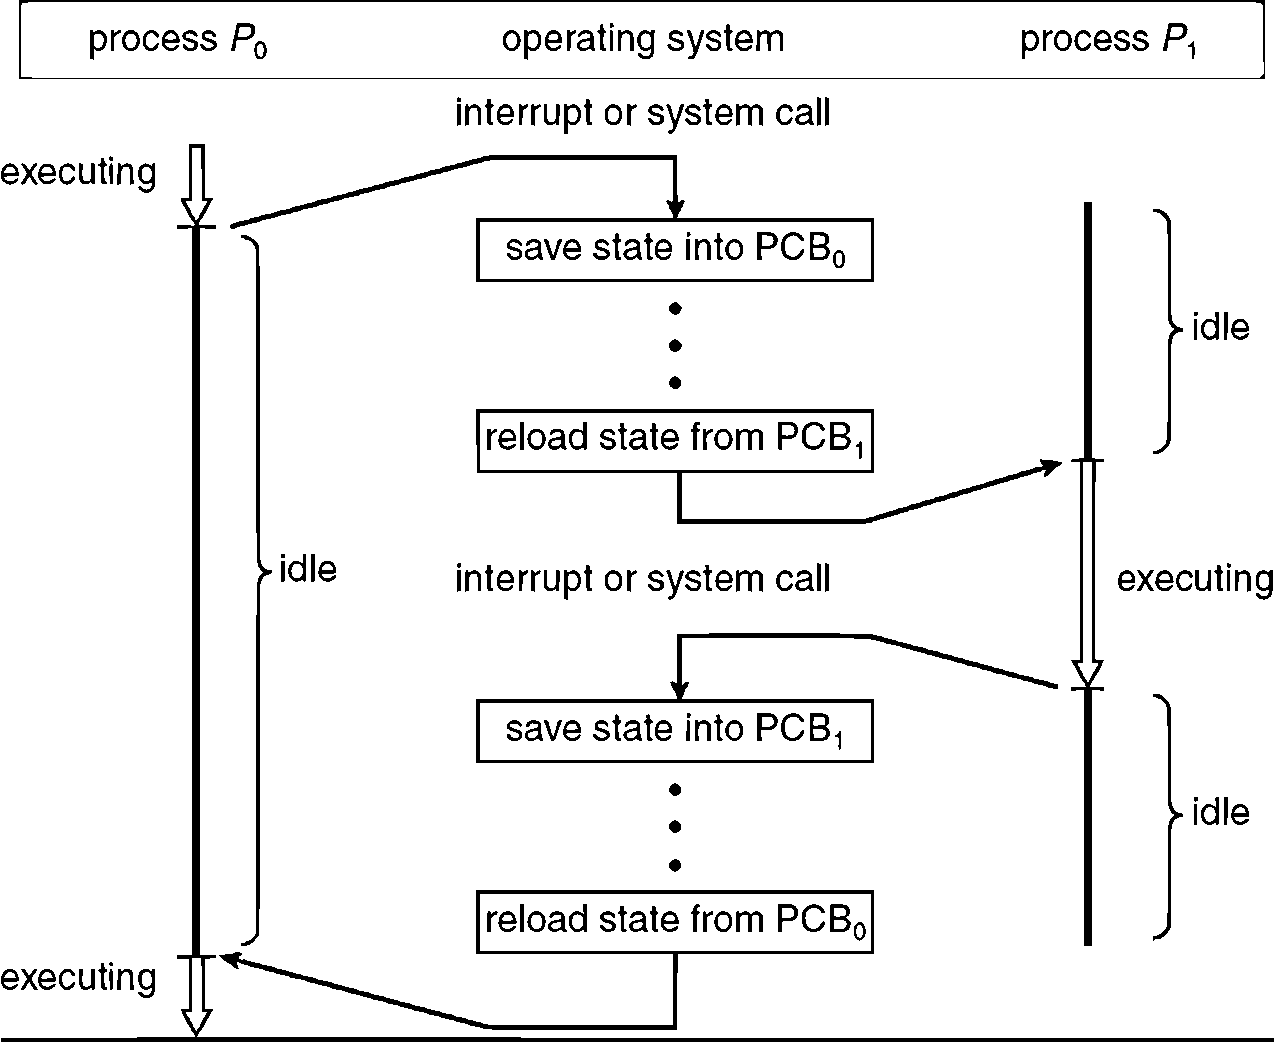
\includegraphics[width=.5\textwidth]{switch}
  \end{center}
  \caption{Context switch}
  \label{fig:ctxt-switch}
\end{figure}

\paragraph{Data Structures For Task Management}

\begin{codeblock}[1]
\begin{ccode}
struct TASKLEVEL
{ 
  int running; /* how many tasks are running */
  int now;     /* which task is currently running */
  struct TASK* tasks[MAX_TASKS_LV]; /* all tasks in one level */
};
\end{ccode}
\end{codeblock}
\begin{itemize}
\item is used to record the status of each task in a level. The definition of level, see
  ~\ref{sec:process-management}.
  
  
\end{itemize}

\begin{codeblock}[1]
\begin{ccode}
struct TSS32
{ 
  int esp0, esp1, esp2; /* stack pointer register */
  int ss0, ss1, ss2;    /* stack segment register */
  int cr3;    /* control register */
  int eip;    /* instruct pointer register */
  int eflags; /* registers flag */
  int eax;    /* accumulator register */
  int ecx;    /* counter register */
  int edx;    /* data register */
  int ebx;    /* base register */
  int esp;    /* stack pointer register */
  int ebp;    /* base pointer register*/
  int esi;    /* source index register */
  int edi;    /* destination index register */
  int es;     /* extra segment register */
  int cs;     /* code segment register */
  int ss;     /* stack segment register */
  int ds;     /* data segment register */
  int fs;     /* segment part 2 */
  int gs;     /* segment part 3 */
  int ldtr;   /* LDT segment selector */
  int iomap;  /* I/O map base address */
};
\end{ccode}
\end{codeblock}
\begin{itemize}
\item holds information about task status segments, which are based on CPU
  specifications\cite[Sec.6.2.1]{intel_3a}. The \emph{eip} register records where in the
  memory the next instruction to be executed by the CPU is located.
\end{itemize}

\begin{codeblock}[1]
\begin{ccode}
struct TASKCTL
{ 
  int now_lv;    /* current activity level */
  int lv_change; /* does the level need to be changed next time the task is switched */
  struct TASKLEVEL level[MAX_TASKLEVELS]; /* all levels*/
  struct TASK tasks0[MAX_TASKS];          /* all running tasks */
};
\end{ccode}
\end{codeblock}
\begin{itemize}
\item is used to control all tasks in the system. This structure uses the \emph{now\_lv}
  variable to record the current running \emph{level} in the system. See
  Fig. ~\ref{fig:proc-manage}.
  
  
\end{itemize}

\begin{codeblock}[1]
\begin{ccode}
struct TASK
{ 
  int sel;              /* the number of GDT */
  int flags;            /* the state of task */
  int level;            /* the level of task */
  int priority;         /* the priority of task */
  struct FIFO32 fifo;   /* a fifo buffer */
  TSS32 tss;            /* TSS segment for a task */
  struct CONSOLE* cons; /* the console window address of task */
  int ds_base;          /* data segment address of APPs */
  int cons_stack;       /* the stack address of APPs */
  struct SEGMENT_DESCRIPTOR ldt[2]; /* tow LDT segments of task */
  struct FILEHANDLE* fhandle; /* file handles for manipulating files */
  int* fat; /* file allocation table */
  char* cmdline; /* store the command line context */
  unsigned char langmode;  /* which font to use */
  unsigned char langbyte1; /* store the first byte of the full-width character */
};
\end{ccode}
\end{codeblock}
\begin{itemize}
\item is used to manage variables for a task. Record the task's sections, permissions,
  stacks, etc. Actually, this is a PCB.
\end{itemize}

\paragraph{Task Management Functions}

\csingle|struct TASK *task_now(void);|
\begin{itemize}
\item Returns the address of which task level of which task is currently running. 
    
\end{itemize}

\csingle|struct TASK *task_init(struct MEMMAN *memman);|
\begin{itemize}
\item Initialize all empty tasks. This
  function will register all 1000 empty tasks to the GDT table. Initialize all levels of
  task running variables \emph{running} to 0. The pointer \emph{now} of each level
  indicating that the task is currently running is also set to 0. In fact, this function
  registers all empty PCBs for future management tasks. At the same time, the task that
  calls this task needs tobe managed so the address of a PCB is returned. An idle task
  needs to be set in the last \emph{level}. Ensure that at least one task is running in the
  system.
  
\end{itemize}

\csingle|struct TASK *task_alloc(void);|
\begin{itemize}
\item Get an empty PCB from the \emph{task pool~\ref{sec:process-management}}. Return
  its address if successful, otherwise 0. 
  
\end{itemize}

\csingle|void task_run(struct TASK *task, int level, int priority);|
\begin{itemize}
\item Add a task to \emph{task pool}. The \emph{level} and \emph{priority} of tasks
  through this function can also be set. If the task is asleep, wake it up. Note that this
  function will not immediately cause the running of task after the execution of this
  function. Instead wait to be scheduled.
\end{itemize}

\csingle|void task_switch(void);|
\begin{itemize}
\item Switch to the next task. This function will select one of the highest \emph{level}
  tasks to run from the \emph{task pool}. 
  
\end{itemize}

\csingle|void task_sleep(struct TASK *task);|
\begin{itemize}
\item Put a task into sleep. The task that is being promoted to sleep may be the currently
  running task in the system. If this is the case, it must also schedule the task in
  the entire \emph{task pool}. Then jump to this new task and start running.
      
\end{itemize}

\subsubsection{Graphic Management}
\label{sec:graphic}

The patterns on the screen belong to one \emph{sheet}. A \emph{sheet} is a structure that
records how a certain height of a certain area of a computer screen should be
displayed. Graphics management is also responsible for refreshing the computer screen when
the content displayed by a \emph{sheet} changes. Graphic management is also responsible
for setting the height of the \emph{sheet}. The \emph{sheet} height setting is a relatively
complex part of the graphics management, which will be explained in detail in the
implementation section. Usually the lowest \emph{sheet} is the computer desktop, which is the
background layer. The highest \emph{sheet} is the mouse layer. In general, for modern
operating systems, graphics management is not a matter of the operating system kernel. So
this part only shows in detail the more complicated part of the \emph{sheet} height
setting. Fig. ~\ref{fig:state-sheets} shows the possible state of some of the \emph{sheet}
on the computer screen.
\begin{figure}[!ht]
  \centering
  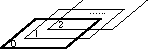
\includegraphics[width=.5\textwidth]{sheets.pdf}
  \caption{a state of sheets}
  \label{fig:state-sheets}
\end{figure}
The figure shows three \emph{sheet} and is labeled 0, 1, 2. Of course there may be more
than three \emph{sheet}. \emph{Sheet} 2 is in the highest position, and \emph{sheet} 0 is
the lowest.


  
\paragraph{Graphic Management Data Structures}

\begin{codeblock}[1]
\begin{ccode}
struct SHEET
{ 
  char* buf;   /* address of the graphic content depicted */
  int bxszie;  /* size of x coordinate of sheet */
  int bysize;  /* size of y coordinate of sheet */
  int vx0;     /* x coordinate of sheet */
  int vy0;     /* y coordinate of sheet */
  int col_inv; /* number of invisible color */
  int height;  /* height of sheet */
  int flags;   /* states of sheet, using or not */
};
\end{ccode}
\end{codeblock}
\begin{itemize}
\item is used to record layer-related information, including the layer's size and
  position.
\end{itemize}

\begin{codeblock}[1]
\begin{ccode}
struct SHTCTL
{ 
  unsigned char* vram; /* the address of VRAM */
  unsigned char* map;  /* which layer the pixel on the screen belongs to*/
  int xsize; /* the x size of screen */
  int ysize; /* the y size of screen */
  int top;   /* the height of the top layer */
  struct SHEET* sheets[MAX_SHEETS]; /* order all layer addresses in order */
  struct SHEET sheets0[MAX_SHEETS]; /* all layers */
};
\end{ccode}
\end{codeblock}
\begin{itemize}
\item is used to manage the structure of multiple layer information, including how many
  layers there are in total, the size and height of each layer.
\end{itemize}

\paragraph{Graphic Management Functions}

\csingle|struct SHTCTL *shtctl_init(struct MEMMAN *memman,unsigned char *vram,int xsize,int ysize);|
\begin{itemize}
\item Initialize a sheet control structure, \emph{vram} is the address of video
  RAM. \emph{xsize} and \emph{ysize} is the size of sheet. Mark all sheet structures
  as 0 to indicate that they are not used.
  
\end{itemize}

\csingle|struct SHEET *sheet_alloc(struct SHTCTL *ctl);|
\begin{itemize}
\item Return a \emph{SHEET} structure if success, otherwise 0. Find an unused \emph{sheet} from
  the sheet structure control structure and making this \emph{sheet} in using.
  
\end{itemize}

\csingle|void sheet_setbuf(struct SHEET *sht,unsigned char *buf,int xsize,int ysize,int col_inv);|
\begin{itemize}
\item Set the properties of the \emph{buf} pf \emph{sheet}. 
\end{itemize}

\csingle|void sheet_updown(struct SHEET *sht, int height);|
\begin{itemize}
\item Set the height of layer \emph{sht}. The height of the \emph{sheet} is more complicated to
  set, which will be explained in detail in the implementation section.
  
  
\end{itemize}

\csingle|void sheet_refresh(struct SHEET *sht, int bx0, int by0, int bx1, int by1);|
\begin{itemize}
\item Refreshes the screen range specified by \emph{bx0}, \emph{by0}, \emph{bx1} and
  \emph{by1}. There are many \emph{sheet} on the computer screen. Not all the ranges of
  all \emph{sheet} will be refreshed when the screen is refreshed. Considering the
  efficiency of the refresh, this also requires a delicate design. But this is generally
  not something that the operating system kernel cares about, so it will be omitted.
\end{itemize}

\csingle|void sheet_free(struct SHEET *sht);|
\begin{itemize}
\item Release a \emph{sheet}. In addition to marking the \emph{sheet} as unused, the first
  thing to do is to hide the \emph{sheet}. 
\end{itemize}

\csingle|void make_window8(unsigned char *buf, int xsize, int ysize, char *title, char act);|
\begin{itemize}
\item Make a window in \emph{SHEET} \emph{buf}. A window is almost indistinguishable from
  a \emph{sheet}. When we create a window, we simply write different data to the
  \emph{buf} of the \emph{sheet} to make it appear as a window.
  
\end{itemize}

\csingle|void putfonts8_asc_sht(struct SHEET *sht, int x, int y, int c, int b, char *s, int l);|
\begin{itemize}
\item Paint the background color \emph{b} and write the characters and finish the
  refreshing. \emph{l} specifies the length of the string \emph{s} to be written.
    
\end{itemize}

\subsubsection{System Calls}
\label{sec:system-call}

The system calls encapsulate each module in the kernel\fxerror{???}. These system calls are part of the
kernel. In this system, system calls are called by the API instead of the
application.\fxerror{see wikipedia}

\paragraph{System Calls Prototype}
\fxerror{more about each function}

\csingle|void cons_putchar(struct CONSOLE *cons, int chr, char move);|
\begin{itemize}
\item put a \emph{chr} character on \emph{cons} console.
\end{itemize}

\csingle|void cons_newline(struct CONSOLE *cons);|
\begin{itemize}
\item newline in \emph{cons} console.
\end{itemize}

\csingle|void cons_putstr0(struct CONSOLE *cons, char *s);|
\begin{itemize}
\item put string \emph{s} in \emph{cons} console, no length.
\end{itemize}

\csingle|void cons_putstr1(struct CONSOLE *cons, char *s, int l);|
\begin{itemize}
\item put string \emph{s} in \emph{cons}, \emph{l} is the length of string
  \emph{s}.
\end{itemize}

\csingle|int cmd_app(struct CONSOLE *cons, int *fat, char *cmdline);|
\begin{itemize}
\item Start an application based on the input from the command line \emph{cmdline};
\end{itemize}

\subsubsection{Driver}
\label{sec:driver}

The device drivers are used to control and manipulate the
hardware. \fxerror*{wikipedia}{The driver blocked the hardware information}. It is the
dividing line between hardware and software. A driver provides a software interface to
hardware devices, enabling operating systems and other computer programs to access
hardware functions without needing to know precise details of the hardware being used.

\paragraph{Driver Functions}

\fxerror{more about each function}
\csingle|void set_palette(int start, int end, unsigned char *rgb);|
\begin{itemize}
\item initialize the palette.
\end{itemize}

\csingle|void init_pic(void);|
\begin{itemize}
\item initialize the PIC.
\end{itemize}

\csingle|void init_keyboard(struct FIFO32 *fifo, int data0);|
\begin{itemize}
\item initialze the keyboard.
\end{itemize}

\csingle|void enable_mouse(struct FIFO32 *fifo, int data0, struct MOUSE_DEC *mdec);|
\begin{itemize}
\item activate mouse.
\end{itemize}

\subsubsection{FAT File System}
\label{sec:fat}

\fxerror*{wikipedia}{The file system defines how data is stored and accessed. The file
  system divides the entire storage space according to a certain form. This facilitates
  the storage of files while increasing the utilization of storage media. The small blocks
  thus divided are called sectors. The FAT records which sectors all files are stored on.}
  
\paragraph{FAT Data Structure}

\begin{codeblock}[1]
\begin{ccode}
struct FILEINFO
{ 
  unsigned char name[8];   /* file name */
  unsigned char ext[3];    /* extend name of file */
  unsigned char type;      /* file attributes */
  char reserve[10];        /* reserve byte */
  unsigned short time;     /* the time for storing file */
  unsigned short date;     /* the date for storing file */
  unsigned short  clustno; /* the file from which sector on the disk is stored */
};
\end{ccode}
\end{codeblock}
\begin{itemize}
\item is used to record file-related information, such as file name, size, etc.
\end{itemize}

\paragraph{FAT Functions}
\fxerror{more about each function}

\csingle|void file_readfat(int *fat, unsigned char *img);|
\begin{itemize}
\item read file allocation table
\end{itemize}

\csingle|void file_loadfile(int clustno, int size, char *buf, int *fat, char *img);|
\begin{itemize}
\item read file contents into memory
\end{itemize}

\csingle|struct FILEINFO *file_search(char *name, struct FILEINFO *finfo, int max);|
\begin{itemize}
\item search for files based on provided \emph{name}.
\end{itemize}

\subsection{API}
\label{sec:api}
In computer programming, APIs are subroutines that are used to develop
applications. Usually, it communicates all parts of the software. A good API makes
application development easier. By abstracting the underlying implementation and only
exposing objects or actions the developer needs, an API simplifies programming.

\subsubsection{All APIs}
\label{sec:all-apis}
\fxerror{more about each function}

\csingle|void api_putchar(int c);|
\begin{itemize}
\item output a character \emph{c} on the console window.
\end{itemize}

\csingle|void api_putstr0(char *s);|
\begin{itemize}
\item ouput a string \emph{s} on the console window.
\end{itemize}

\csingle|void api_putstr1(char *s, int l);|
\begin{itemize}
\item output a string \emph{s} on console window, \emph{l} is the length of this string.
\end{itemize}

\csingle|void api_end(void);|
\begin{itemize}
\item end the application's running.
\end{itemize}

\csingle|int api_openwin(char *buf, int xsiz, int ysiz, int col_inv, char *title);|
\begin{itemize}
\item open a window, return the hanlder of window.
\end{itemize}

\csingle|void api_putstrwin(int win, int x, int y, int col, int len, char *str);|
\begin{itemize}
\item display string \emph{str} on window. 
\end{itemize}

\csingle|void api_boxfilwin(int win, int x0, int y0, int x1, int y1, int col);|
\begin{itemize}
\item draw a box on the window
\end{itemize}

\csingle|void api_initmalloc(void);|
\begin{itemize}
\item initialize the structure of the management memory
\end{itemize}

\csingle|char *api_malloc(int size);|
\begin{itemize}
\item allocating memory for the application.
\end{itemize}

\csingle|void api_free(char *addr, int size);|
\begin{itemize}
\item free up memory used by the application.
\end{itemize}

\csingle|void api_point(int win, int x, int y, int col);|
\begin{itemize}
\item draw a pint on \emph{win} window.
\end{itemize}

\csingle|void api_refreshwin(int win, int x0, int y0, int x1, int y1);|
\begin{itemize}
\item refresh the window.
\end{itemize}

\csingle|void api_linewin(int win, int x0, int y0, int x1, int y1, int col);|
\begin{itemize}
\item draw a straight line.
\end{itemize}

\csingle|void api_closewin(int win);|
\begin{itemize}
\item close window.
\end{itemize}

\csingle|int api_getkey(int mode);|
\begin{itemize}
\item accept keyboard input.
\end{itemize}

\csingle|int api_alloctimer(void);|
\begin{itemize}
\item get timer.
\end{itemize}

\csingle|void api_inittimer(int timer, int data);|
\begin{itemize}
\item set the data of timer sending.
\end{itemize}

\csingle|void api_settimer(int timer, int time);|
\begin{itemize}
\item set the time of timer.
\end{itemize}

\csingle|void api_freetimer(int timer);|
\begin{itemize}
\item release timer.
\end{itemize}

\csingle|void api_beep(int tone);|
\begin{itemize}
\item make a buzzer sound
\end{itemize}

\csingle|int api_fopen(char *fname);|
\begin{itemize}
\item open file, return file hanlder
\end{itemize}

\csingle|void api_fclose(int fhandle);|
\begin{itemize}
\item close file
\end{itemize}

\csingle|void api_fseek(int fhandle, int offset, int mode);|
\begin{itemize}
\item locate a file
\end{itemize}

\csingle|int api_fsize(int fhandle, int mode);|
\begin{itemize}
\item return the size of \emph{fhandle} file.
\end{itemize}

\csingle|int api_fread(char *buf, int maxsize, int fhandle);|
\begin{itemize}
\item read file, return read bytes. 
\end{itemize}

\csingle|int api_cmdline(char *buf, int maxsize);|
\begin{itemize}
\item return the context of command line.
\end{itemize}

\csingle|int api_getlang(void);|
\begin{itemize}
\item return the language mode.
\end{itemize}

\subsection{APPs}
\label{sec:apps-1}
Since this design is only about the operating system itself, only three representative
applications are introduced. The first is the application of the display color:
\emph{color}. The second is the application for timing: \emph{sundial}. The third
application is to imitate the application of stars in the sky: \emph{stars2}.

\iffalse %%%%%%%%%%%%%%%%%%%%%%%%%%%%%%%%%%%%%%%%%%%%%%%%%%%%%%%%%%%%%%%%%%%%%%%%%%%%%%%%%%%%%%%%%%
\subsubsection{1. Data Structure in Kernel}
In this section data structures used in the RongOS operating system will be introduced in
detail.

\paragraph{BOOTINFO}

\begin{listing}[H]
  \begin{codeblock}
\begin{ccode}
struct BOOTINFO
{
  char cyls;          /* how many cylinder should be read */
  char leds;          /* the status of LED on keyboard */
  char vmode;         /* the mode of video card */
  char reserve;
  short scrnx, scrny; /* resolution of screen */
  char *vram;
};
\end{ccode}
  \end{codeblock}
  \caption{\emph{struct BOOTINFO}}\label{src:bootinfo}
\end{listing}

(code~\ref{src:bootinfo}) is used to store startup-related
information, such as how many cylinders were read, the status of the keyboard indicator,
the mode of the screen, the size of the screen, and the memory address of the graphics
card.


\paragraph{FIFO32}

\begin{listing}[H]
  \begin{codeblock}
\begin{ccode}
struct 
{ 
  int* buf;          /* the address of FIFO32 buffer */
  int p;             /* the writing address */
  int q;             /* the reading address */
  int size;          /* the size of FIFO32 buffer */
  int free;          /* how many space free */
  int flags;         /* the states of FIFO32 buffer */
  struct TASK* task; /* point to a task */ 
};
\end{ccode}
  \end{codeblock}
  \caption{\emph{struct FIFO32}}\label{src:FIFO32}
\end{listing}

(code~\ref{src:FIFO32}) is used to
describe a FIFO structure. This structure is used to receive various kinds of
information. It specifies where to read and write the FIFO structure and the size of the
buffer, available size.


\paragraph{SEGMENT\_DESCRIPTOR}

\begin{listing}[H]
  \begin{codeblock}
\begin{ccode}
struct 
{ 
  short limit_low;   /* the low part of segment size */
  short base_low;    /* the low part of base address */
  char base_mid;     /* the middle part of base address */
  char access_right; /* read and write permissions etc */
  char  limit_high;  /* the high part of segment size */
  char base_high;    /* the high part of base address */
};
\end{ccode}
  \end{codeblock}
  \caption{\emph{struct SEGMENT\_DESCRIPTOR}}\label{src:DESCRIPTOR}
\end{listing}

(code~\ref{src:DESCRIPTOR}) structure is
used to store GDT related information, which is based on CPU specifications(3.5.1 and
3.4.5\cite{intel_3a}). GDT is stored at 270000 in memory.


\paragraph{GATE\_DESCRIPTOR}

\begin{listing}[H]
  \begin{codeblock}
\begin{ccode}
struct 
{ 
  short offset_low;   /* the low part of offset */
  short selector;     /* which interrupt to choose */
  char dw_count;      /* how many interrupts are registered */
  char access_right;  /* access permission */
  short  offset_high; /* high part of offset */
};
\end{ccode}
  \end{codeblock}
  \caption{\emph{struct GATE\_DESCRIPTOR}}\label{src:GATEDESCRIPTOR}
\end{listing}

(code~\ref{src:GATEDESCRIPTOR}) structure is used to
store IDT related information, which is based on CPU specifications(3.5.1 and
3.4.5\cite{intel_3a}). IDT is at 26f800 memory.


\paragraph{MOUSE\_DEC}

\begin{listing}[H]
  \begin{codeblock}
\begin{ccode}
struct 
{ 
  unsigned char buf[3]; /* store the data from mouse */
  unsigned char phase;  /* the stage of receiving mouse data */
  int x;                /* the x point of mouse */
  int y;                /* the y point of mouse */
  int btn;              /* whether the mouse is pressed */
};
\end{ccode}
  \end{codeblock}
  \caption{\emph{struct MOUSE\_DEC}}\label{src:MOUSE}
\end{listing}

(code~\ref{src:MOUSE}) structure is used to store information about the mouse, such as the
location of the mouse, whether the mouse is pressed or not.

\paragraph{FREEINFO}

\begin{listing}[H]
  \begin{codeblock}
\begin{ccode}
struct 
{ 
  unsigned int addr; /* the starting address of free space */
  unsigned int size; /* how many size is free */
};
\end{ccode}
  \end{codeblock}
  \caption{\emph{struct FREEINFO}}\label{src:FREEINFO}
\end{listing}

(code~\ref{src:FREEINFO}) structure stores how many bytes are
free from where in memory.




\paragraph{MEMMAN}

\begin{listing}[H]
  \begin{codeblock}
\begin{ccode}
struct 
{ 
  int frees;                           /* how many memory blocks are free */
  int maxfrees;                        /* the maximum of frees */
  int lostsize;                        /* release the sum of the failed memory size */
  int losts;                           /* the number of failures */
  struct FREEINFO free[MEMMAN_FREES];  /* record all free memory block information */
};
\end{ccode}
  \end{codeblock}
  \caption{\emph{struct MEMMAN}}\label{src:MEMMAN}
\end{listing}

(code~\ref{src:MEMMAN}) structure is used to store the entire memory usage, such as the total
remaining memory space and entries.



\paragraph{SHEET}

\begin{listing}[H]
  \begin{codeblock}
\begin{ccode}
struct 
{ 
  char* buf;   /* the address of the graphic content depicted */
  int bxszie;  /* the size of x coordinate of sheet */
  int bysize;  /* the size of y coordinate of sheet */
  int vx0;     /* the x coordinate of sheet */
  int vy0;     /* the y coordinate of sheet */
  int col_inv; /* the number of invisible color */
  int height;  /* the height of sheet */
  int flags;   /* the states of sheet, using or not */
};
\end{ccode}
  \end{codeblock}
  \caption{\emph{struct SHEET}}\label{src:SHEET}
\end{listing}

(code~\ref{src:SHEET}) structure is used to store the entire memory usage, such as the
total remaining memory space and entries.



\paragraph{SHTCTL}

\begin{listing}[H]
  \begin{codeblock}
\begin{ccode}
struct 
{ 
  unsigned char* vram;              /* the address of VRAM */
  unsigned char* map;               /* which layer the pixel on the screen belongs to*/
  int xsize;                        /* the x size of screen */
  int ysize;                        /* the y size of screen */
  int top;                          /* the height of the top layer */
  struct SHEET* sheets[MAX_SHEETS]; /* order all layer addresses in order */
  struct SHEET sheets0[MAX_SHEETS]; /* all layers */
};
\end{ccode}
  \end{codeblock}
  \caption{\emph{struct SHTCTL}}\label{src:SHTCTL}
\end{listing}

(code~\ref{src:SHTCTL}) structure is used to manage the structure of multiple layer information,
including how many layers there are in total, the size and height of each layer.



\paragraph{TIMER}

\begin{listing}[H]
  \begin{codeblock}
\begin{ccode}
struct 
{ 
  struct TIMER* next;   /* the next timer that is about to timeout */
  unsigned int timeout; /* how long is the timeout */
  char flags;           /* the states of timer */
  char flgas2;          /* whether to allow automatic cancellation */
  struct FIFO32* fifo;  /* store data(from mouse, keyboard etc) */
  int data;             /* accept data */
};
\end{ccode}
  \end{codeblock}
  \caption{\emph{struct TIMER}}\label{src:TIMER}
\end{listing}

(code~\ref{src:TIMER}) structure is used to manage the time slice of the CPU. The timer
interrupts the CPU at regular intervals. This structure records the length of the timer,
usage status and other information.



\paragraph{TIMERCTL}

\begin{listing}[H]
  \begin{codeblock}
\begin{ccode}
struct 
{ 
  unsigned int count;   /* count variable */
  unsigned int next;    /* the next timeout timer */
  sturct TIMER* t0;     /* the shortest timeout timer */
  struct TIMER timers0; /* all timers */
};
\end{ccode}
  \end{codeblock}
  \caption{\emph{struct TIMERCTL}}\label{src:TIMERCTL}
\end{listing}

(code~\ref{src:TIMERCTL}) structure is used to manage all timers in the system. Including
how many timers are in total, current use, and the next timer to be used.



\paragraph{TSS32}

\begin{listing}[H]
  \begin{codeblock}
\begin{ccode}
struct 
{ 
  int esp0, esp1, esp2; /* stack pointer register */
  int ss0, ss1, ss2;    /* stack segment register */
  int cr3;              /* control register */
  int eip;              /* instruct pointer register */
  int eflags;           /* registers flag */
  int eax;              /* accumulator register */
  int ecx;              /* counter register */
  int edx;              /* data register */
  int ebx;              /* base register */
  int esp;              /* stack pointer register */
  int ebp;              /* base pointer register*/
  int esi;              /* source index register */
  int edi;              /* destination index register */
  int es;               /* extra segment register */
  int cs;               /* code segment register */
  int ss;               /* stack segment register */
  int ds;               /* data segment register */
  int fs;               /* segment part 2 */
  int gs;               /* segment part 3 */
  int ldtr;             /* LDT segment selector */
  int iomap;            /* I/O map base address */
};
\end{ccode}
  \end{codeblock}
  \caption{\emph{struct TSS32}}\label{src:TSS32}
\end{listing}

(code~\ref{src:TSS32}) structure holds information about task status segments, which are
based on CPU specifications(See 6.2.1\cite{intel_3a}).


\paragraph{FILEHANDLE}

\begin{listing}[H]
  \begin{codeblock}
\begin{ccode}
struct 
{ 
  char* buf; /* store the handler of file */
  int size;  /* the size of file */
  int pos;   /* where to read the file */
};
\end{ccode}
  \end{codeblock}
  \caption{\emph{struct FILEHANDLE}}\label{src:FILEHANDLE}
\end{listing}

(code~\ref{src:FILEHANDLE}) is used to record an open file related data structure.



\paragraph{TASK}

\begin{listing}[H]
  \begin{codeblock}
\begin{ccode}
struct 
{ 
  int sel;                          /* the number of GDT */
  int flags;                        /* the state of task */
  int level;                        /* the level of task */
  int priority;                     /* the priority of task */
  struct FIFO32 fifo;               /* a fifo buffer */
  TSS32 tss;                        /* TSS segment for a task */
  struct CONSOLE* cons;             /* the console window address of task */
  int ds_base;                      /* data segment address of APPs */
  int cons_stack;                   /* the stack address of APPs */
  struct SEGMENT_DESCRIPTOR ldt[2]; /* tow LDT segments of task */
  struct FILEHANDLE* fhandle;       /* file handles for manipulating files */
  int* fat;                         /* file allocation table */
  char* cmdline;                    /* store the command line context */
  unsigned char langmode;           /* which font to use */
  unsigned char langbyte1;          /* store the first byte of the full-width character */
};
\end{ccode}
  \end{codeblock}
  \caption{\emph{struct TASK}}\label{src:TASK}
\end{listing}

(code~\ref{src:TASK})is used to manage variables for a task. Record the task's sections,
permissions, stacks, etc.


\paragraph{TASKLEVEL}

\begin{listing}[H]
  \begin{codeblock}
\begin{ccode}
struct 
{ 
  int running;                      /* how many tasks are running */
  int now;                          /* which task is currently running */
  struct TASK* tasks[MAX_TASKS_LV]; /* all tasks in one level */
};
\end{ccode}
  \end{codeblock}
  \caption{\emph{struct TASKLEVEL}}\label{src:TASKLEV}
\end{listing}

(code~\ref{src:TASKLEV}) is used to record the status of each task in a layer.


\paragraph{TASKCTL}

\begin{listing}[H]
  \begin{codeblock}
\begin{ccode}
struct 
{ 
  int now_lv;    /* current activity level */
  int lv_change; /* does the hierarchy need to be changed next time the task is switched */
};
\end{ccode}
  \end{codeblock}
  \caption{\emph{struct TASKCTL}}\label{src:TASKCT}
\end{listing}

(code~\ref{src:TASKCT}) is used to control all tasks in the system.



\paragraph{CONSOLE}

\begin{listing}[H]
  \begin{codeblock}
\begin{ccode}
struct 
{ 
  struct SHEET* sht;   /* which layer is used on the command line */
  int cur_x;           /* the x position of console */
  int cur_y;           /* the y position of console */
  int cur_c;           /* the color of console */
  struct TIMER* timer; /* timer to control cursor blinking */
};
\end{ccode}
  \end{codeblock}
  \caption{\emph{struct CONSOLE}}\label{src:CONSOLE}
\end{listing}

(code~\ref{src:CONSOLE})is used to record information about a console terminal, such as location,
color, and so on.




\paragraph{FILEINFO}

\begin{listing}[H]
  \begin{codeblock}
\begin{ccode}
struct
{ 
  unsigned char name[8];   /* file name */
  unsigned char ext[3];    /* extend name of file */
  unsigned char type;      /* file attributes */
  char reserve[10];        /* reserve byte */
  unsigned short time;     /* the time for storing file */
  unsigned short date;     /* the date for storing file */
  unsigned short  clustno; /* the file from which sector on the disk is stored */
};
\end{ccode}
  \end{codeblock}
  \caption{\emph{struct FILEINFO}}\label{src:FILEINFO}
\end{listing}

(code~\ref{src:FILEINFO}) is used to record file-related information, such as file name, size,
etc.
\fi %%%%%%%%%%%%%%%%%%%%%%%%%%%%%%%%%%%%%%%%%%%%%%%%%%%%%%%%%%%%%%%%%%%%%%%%%%%%%%%%%%%%%%%%%%%%%%%%%%%%%%%


    
%\subsection{API}
%\label{sec:api}

%\subsection{APPs}
%\label{sec:apps-1}



\chapter{Implementation}

\section{Boot Up}
\label{sec:boot-up-1}

The boot loader is implemented in Intel assembly. It works as follows:

\begin{enumerate}
\item \textbf{Display boot information:} Firstly, the code in boot sector (See
  Appendix~\ref{sec:dis-boo-inf}) outputs some boot information. \fxerror*{Not clear. You
    have to explain what is al/ah for. For example, as shown in table... al is for..., ah
    is for... int 0x10 is for...}{When \emph{al=0}, the
  null character of boot information hit. Interrupt \emph{0x10} is used for showing a
  character on the screen.}
\item \textbf{Read the second sector:} Then jump to load C0-H0-S2, \emph{ax} register
  saved the address where beginning puts the sectors from floppy. And preparing parameters
  for interrupt \emph{0x13} in registers. The \emph{0x13} interrupt used for read
  sector from floppy to memory. (See Appendix~\ref{sec:rea-sec-sec}).
\item \textbf{Read two sides of a track:}
  
  If there is a carry indicating some thing went wrong while reading the floppy disk,
  reset the registers and try reading it again. The read process aborts after five
  unsuccessful read.

  Register \emph{si} is a counter. If no carry (success), jump to next segment, as one
  sector has been read into memory already. The address should increase 512 byte. Then
  sector number (\emph{cl} register) is added by 1 and compare it to 18, if it's smaller
  than 18, jump to \emph{readloop}, read the next sector.

  If the value of \emph{cl} register is bigger or equal to 18, meaning that one track
  18 sector in this side of floppy read already, then reversed the head, add 1 to
  \emph{dh} register.

  If the value of \emph{dh} register after adding larger than or equal to 2, it's saying
  the original head is 1, one track of two sides read already. Otherwise the value of
  \emph{dh} register smaller than 2, read this side indicating by \emph{dh} register,
  jump to \emph{readloop} segmentation. Appendix~\ref{sec:rea-two-sid} is the code 
  performing this function.

  There is a pseudo code about this process:
  \begin{figure}[!ht]
    \centering
    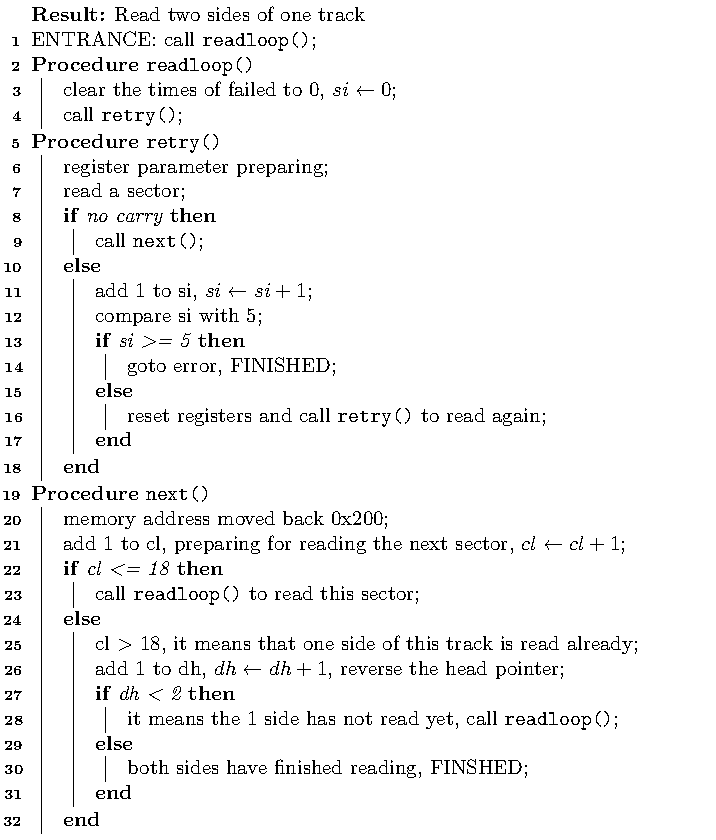
\includegraphics[width=.7\textwidth]{./figs/algorithm/read_two_side.pdf}
    \caption{algorithm of read two sides of one track}
    \label{fig:read_two_sides}
  \end{figure}

  
  
\item \textbf{The next cylinder:} So the next step is moving a cylinder, add 1 to register
  \emph{ch}. Otherwise the value of \emph{dh} register smaller than 2, read this side
  indicating by \emph{dh} register, jump to \emph{readloop} segmentation. After
  \emph{ch} register add 1, if it's smaller than 10, jump to \emph{readloop},
  otherwise end loading floppy to memory process, for we only load ten cylinders of
  floppy. Appendix~\ref{sec:the-nex-cyl} is the code to perform this function.
\end{enumerate}

The above four steps can be intuitively reflected in the Fig. ~\ref{fig:iplflowchart}.
\begin{figure}[!htbp]
  \centering
  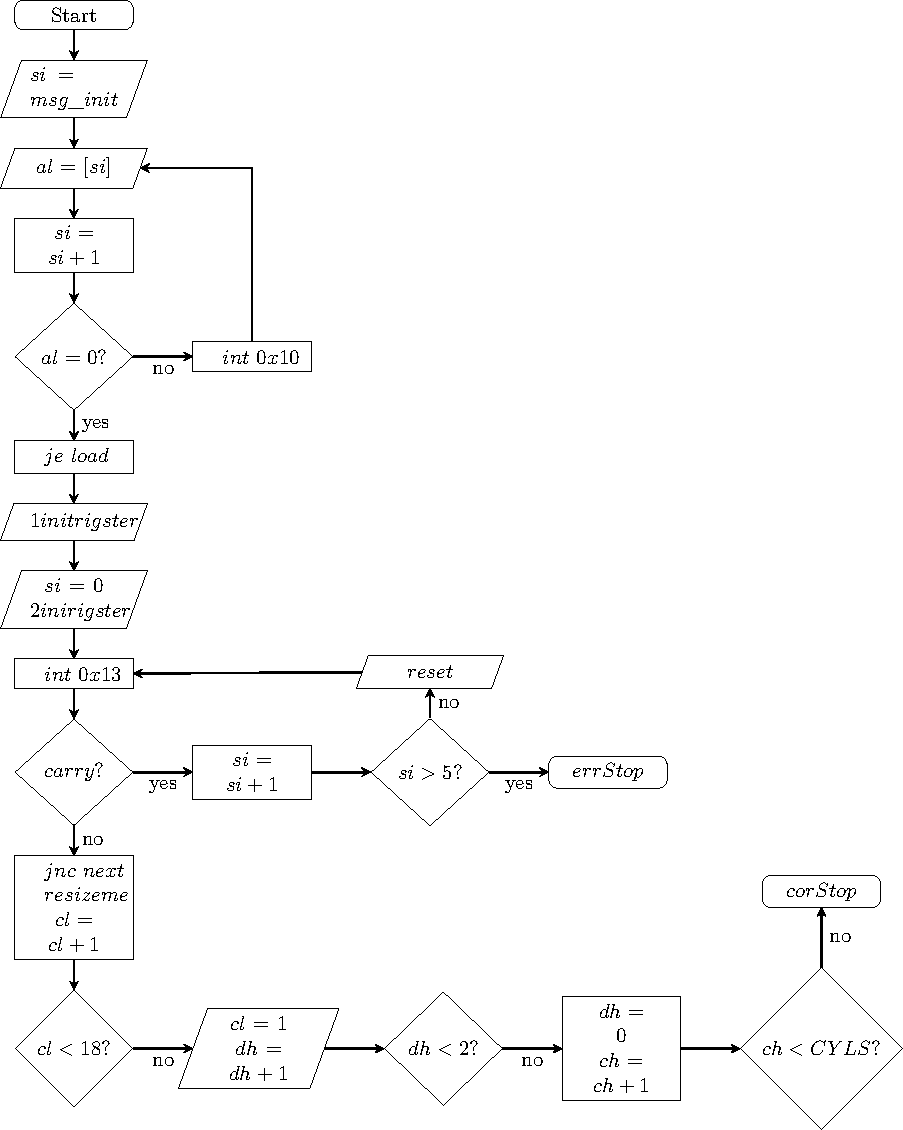
\includegraphics[width=1\textwidth]{flowchartp}
  \caption{the working flowchart of boot loader}
  \label{fig:iplflowchart}
\end{figure}

\section{Kernel}
\label{sec:kernel-1}

\subsection{Memory Management}
\label{sec:memory-management-2}

\subsubsection{Memory Check}
\label{sec:memory-check}

For memory management, memory must be checked to see how large the memory is. After i486,
the CPU turned on the cache function. In order to avoid checking the cache, the CPU's
cache function must be turned off. So first check the version of the CPU. Then check the
memory capacity. When checking the memory capacity, first write a value to the same
address and immediately read out whether the observation is equal to the previously
written value. The entire inspection process can be summarized as follows.
\begin{enumerate}
\item Check the version of the CPU.
\item If the version of the CPU is greater than 386 then caching is disabled, otherwise
  nothing will be done.
  
\item Check memory
\item If the CPU version is greater than the 386 restore cache feature. Otherwise do
  nothing.
\end{enumerate}
Step 2 can be divided into the following steps
\begin{enumerate}
\item Save the original value of a location in memory.
\item Write a constant to the above memory address.
\item Read the above memory address and invert it.
\item The inverted value of the constant prepared in advance is compared with the value
  obtained in the third step.
\item Equal to continue to check, otherwise stop.
\end{enumerate}
In general, the C compiler has optimized optimization, so it seems that the above
comparison is definitely equivalent. So the above check subfunction should be done in
assembly language. Specific implementation, please see appendix
~\ref{sec:memory-check-process}.

\subsubsection{Memory Allocation}
\label{sec:memory-allocation}
First explain some of the variables used to implement the memory allocation
function. \emph{size} refers to the space requested by the application but \emph{SIZE}
is the free space of one \emph{entry}. \emph{free} is the number of memory available
memory.

\begin{enumerate}
\item Traversing all the free entries in memory to find an \emph{entry} gives it more free space
  than the application requested. If found then 2, otherwise 6.
\item Add \emph{size} to start address of \emph{entry} found in 1. Subtract 
  \emph{size} from free space \emph{SIZE} in \emph{entry} found in 1. Jump to 3.
\item Determine if the remaining free space \emph{SIZE} in the entry is 0. If so, go to
  4. Otherwise 5.
\item Subtract the number of memory available entries \emph{free} by 1.
\item Returns the starting address of available memory.
\item Returns 0 for memory allocation failure.
\end{enumerate}
Specific implementation see code ~\ref{sec:memory-alloc-proc}.

\subsubsection{Memory Release}
\label{sec:memory-release}

Memory release is a more complex part of memory management. In order to keep the memory
free entries in an orderly manner and merge adjacent entries, the memory release code
becomes somewhat complicated. It is mainly divided into the following categories.
\begin{enumerate}
\item Neither merge with the previous \emph{entry} nor with the latter \emph{entry}. For
  this case, this entry needs to be inserted into the free memory entry. As the figure
  ~\ref{fig:no-merge} shows.
  \begin{figure}[!ht]
    \centering
    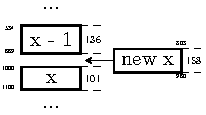
\includegraphics[width=.6\textwidth]{no_merge}
    \caption{insert an entry no merge}
    \label{fig:no-merge}
  \end{figure}
  As shown in the figure, the starting address of \emph{new x} 803 is not adjacent to
  the previous termination address 669, and its termination address 960 is also not
  adjacent to the starting address 1000 of the next entry. The so-called neighboring means
  that the difference between the two addresses is 1. Same as below.

\item Can be merged with the previous entry. As the figure ~\ref{fig:former-merge} shows.
  \begin{figure}[!ht]
    \centering
    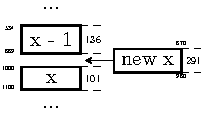
\includegraphics[width=.6\textwidth]{former_merge}
    \caption{Insert an item merged with the previous item}
    \label{fig:former-merge}
  \end{figure}
  As shown in the figure, the starting address of \emph{new x} 670 is adjacent to the
  previous termination address 669, but its termination address 960 is not adjacent to the
  starting address 1000 of the next entry.


\item Can be merged with the latter entry. As the figure ~\ref{fig:latter-merge} shows.
  \begin{figure}[!ht]
    \centering
    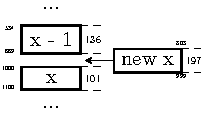
\includegraphics[width=.6\textwidth]{latter_merge}
    \caption{Insert an item merged with the latter item}
    \label{fig:latter-merge}
  \end{figure}
  The termination address 999 of \emph{new x} is adjacent to the starting address 1000
  of the next entry, but its starting address of \emph{new x} 803 is not adjacent to the
  previous termination address 669.
  
\end{enumerate}
The memory release process can be described as follows.
\begin{enumerate}
\item Find the insertion position \emph{i}. The so-called insertion position is an \emph{entry}
  number that satisfies certain conditions. This condition is that the \emph{size} of this
  \emph{entry} is larger than the size requested by the application.
\item If $i > 0$, merge if the newly inserted \emph{entry} can be merged with the previous \emph{entry},
  the same as for the latter \emph{entry}. As long as it merges with the former, the
  function returns 0 and the release is successful. Otherwise jump to 3.
\item The program proceeds here so that the newly inserted \emph{entry} must not be
  merged with the previous \emph{entry}. Now check if the newly inserted \emph{entry}
  can be merged with the latter \emph{entries}. If so, merges it and return 0. Otherwise
  jump to 4.
\item The program proceeds here to represent that the newly inserted \emph{entry} cannot be
  merged with any of the entries. Now check the number of used entries with 4090. If the
  former is less than the latter, move all items after the i'th item back one position to
  make room for new items. Then insert this new \emph{entry}. Otherwise jmup to 5.

\item Failed to release, return -1.
\end{enumerate}
The above release process can be explained by the algorithm ~\ref{fig:mem-relase-algo}. Of
course, the flow chart ~\ref{fig:mem-relase-flow} will be more clear. For specific code
implementation, see ~\ref{sec:memory-rele-proc}


\begin{figure}[!ht]
  \centering
  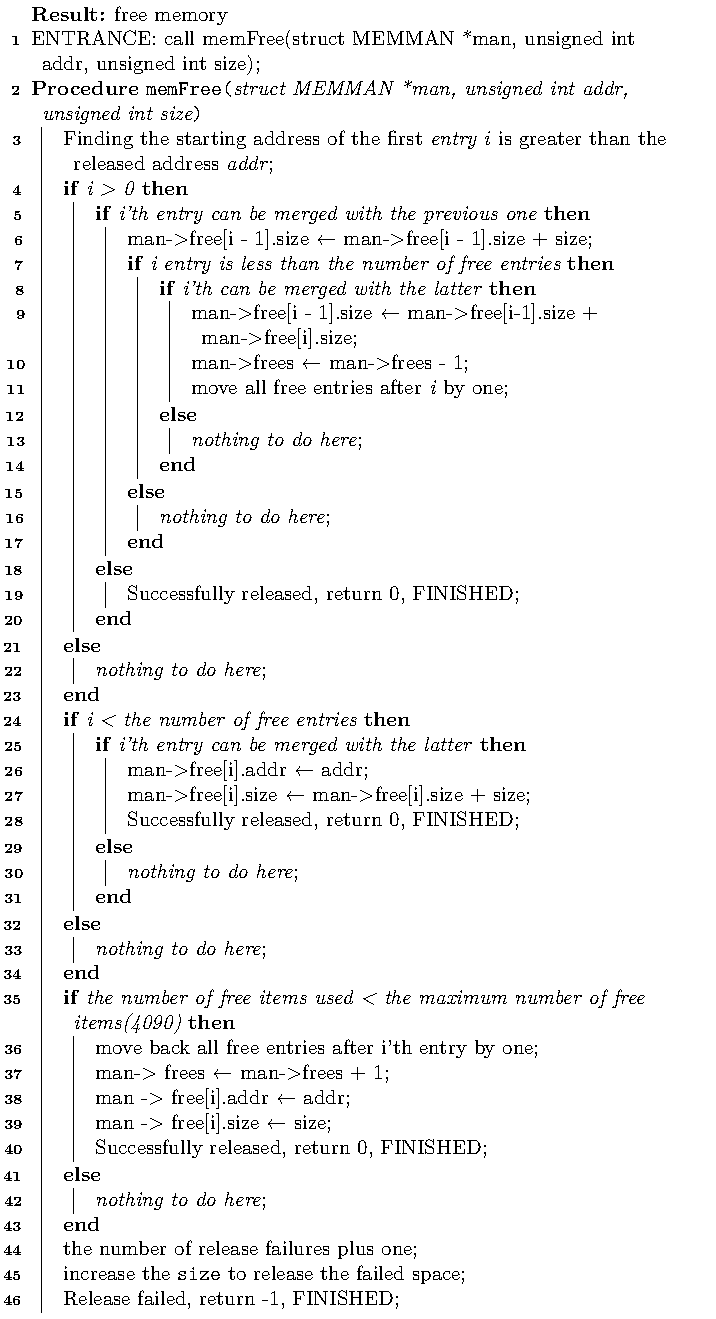
\includegraphics[width=0.8\textwidth]{mem_free}
  \caption{algorithm of release memory}
  \label{fig:mem-relase-algo}
\end{figure}

\begin{figure}[!ht]
  \centering
  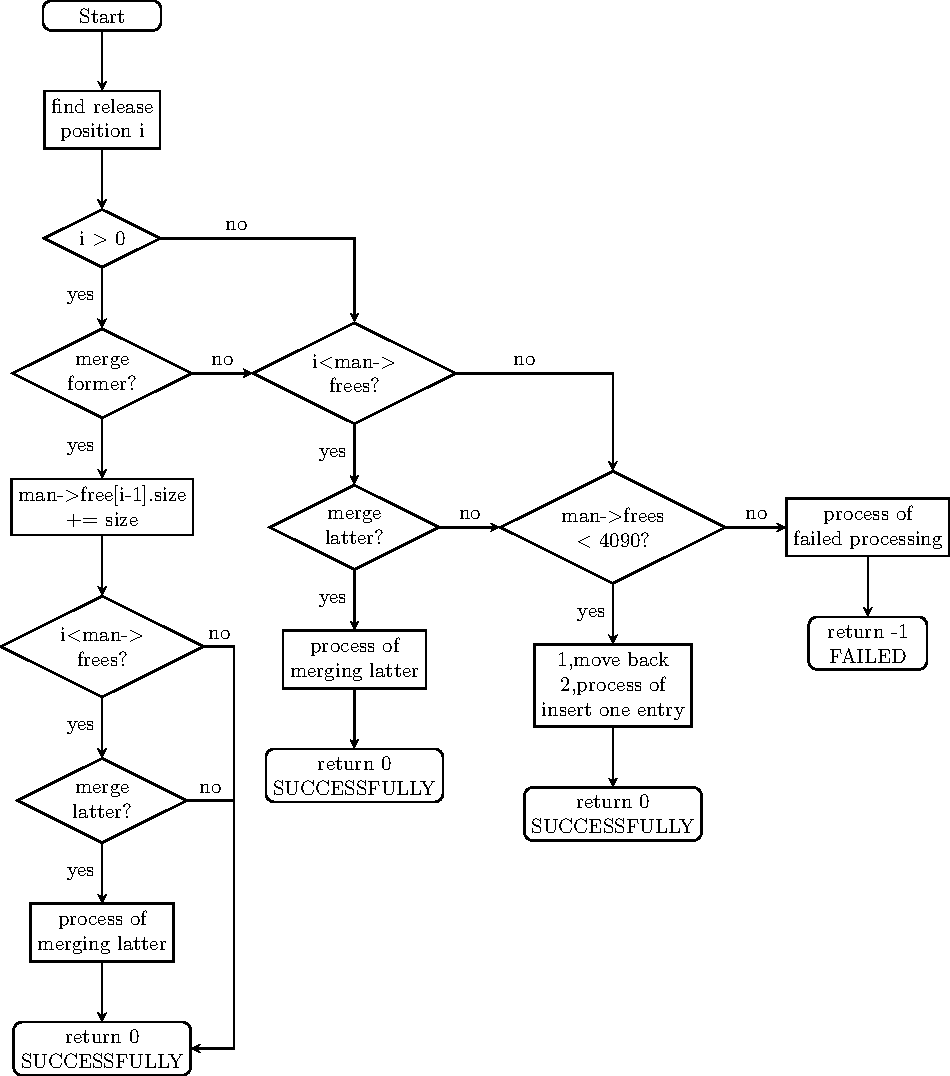
\includegraphics[width=.7\textwidth]{mem_free_flow}
  \caption{flow chart of relase memory}
  \label{fig:mem-relase-flow}
\end{figure}

\subsection{Process Management}
\label{sec:process-management}

Process management is a very complex but very important part of operating system
development. This part of the development has a very big impact on the performance of the
entire system. For the RongOS operating system, all tasks are managed
hierarchically. Fig. ~\ref{fig:proc-manage} clearly shows how all the tasks in the system
are managed.



\begin{figure}[!ht]
  \centering
  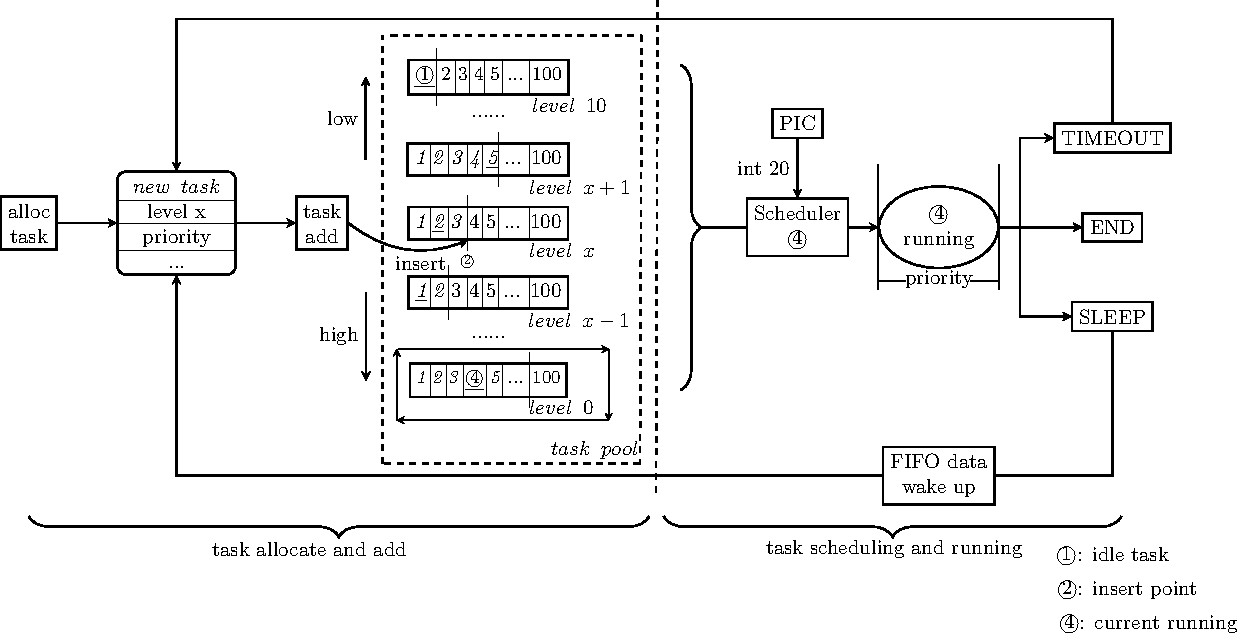
\includegraphics[width=1.1\textwidth]{process-manage}
  \caption{process of task management}
  \label{fig:proc-manage}
\end{figure}



From \emph{level 0} to \emph{level 10}, there are a total of ten levels in
the system. All these ten levels and the space they prepare for the task are called \emph{task
  pool}. For each task, it also has a \emph{priority} attribute. It actually specifies how
long each process can run, also known as a \emph{time slice}. 


As Fig. ~\ref{fig:proc-manage} shows, each level can hold 100 tasks. The lower the
level number, the higher the level's privilege. For example, \emph{x-level} permissions are
higher than \emph{x+1}. The scheduler will select the task to run from a high-privilege
level. Only lower-level tasks are scheduled when the task at the higher privilege level is
completed. While tasks within the same layer are run in turn, their running time may be
different, that is,  the \emph{time slice} is also called \emph{priority}. This can be
illustrated by the peripheral loop arrows in \emph{level 0} in
Fig. ~\ref{fig:proc-manage}. The other \emph{levels} are also similar except that the
peripheral loop arrows are ignored.



In Fig. ~\ref{fig:proc-manage}, a task is added to its corresponding
level. There are many tasks in each level waiting for scheduling or a running task. Tasks
that are waiting for scheduling are represented in italics but the task being run is
underlined in each level. A place after the last task waiting to be scheduled is the
\emph{insertion point} of a new task at a certain level.


The PIC chip will generate 100 clock interrupts per second. Each time a clock interrupt
occurs, it is serviced by the interrupt service routine 0x20. This subroutine will call
the scheduler to schedule a task to run based on the above method of selecting the task to
run. When a run is completed in one round, there are three destinations for a process.
\begin{enumerate}
\item The task did not complete, but the \emph{time slice} was used up. It will be added
  to the task pool again and wait for it to be selected again to begin another run.
\item The task completes the run and then enters the end processing subroutine.
\item The \emph{time slice} of the process runs out, but it goes to \emph{sleep}. The
  so-called \emph{sleep} state means that the process is paused, waiting for something to
  happen and waking it up again, adding it to the \emph{task pool} and starting a round of
  running. Something such as a keyboard input program waits for user input.
  
\end{enumerate}

As shown in Fig. ~\ref{fig:proc-manage}, it can be seen as a snapshot of all the tasks in
the system. In this transient state, a task is being added to the $(3+1=4)$ point of
\emph{x-level} of \emph{task pool}. What is running in the system is task \textcircled{4}
of \emph{level 0}. 


\subsubsection{Task Allocate and Add}
\label{sec:task-allocate-add}
After the new process arrives, it must apply for a task structure to record its
information. This process is simpler simply by iterating through the \emph{tasks0} structure array
variable to find an unused task structure and assign it to the new task. \emph{tasks0} is
used to record information for all tasks. At the same time put the address of this
structure into the \emph{tasks} structure array. This structure \emph{tasks} is used to
record the addresses of all tasks. Note that \emph{tasks} and \emph{tasks0} are
functionally different arrays of structures. \emph{tasks0} records information for all
1000 tasks in the system, while \emph{tasks} record their addresses.


The next step is to add to the \emph{task pool} and wait to be scheduled. When adding,
specify the \emph{level} and \emph{priority}. The specified \emph{level} and
\emph{priority} may not be the same as the original task, or they may be the
same. Different situations need to be handled differently. This can be done by the
following steps.

\begin{enumerate}
\item If the \emph{level} passed in is less than 0, it means that the task is added without
  changing the \emph{level} of the task, and the \emph{level} of the original task is used
  to cover the incoming level. The check here is mainly for processing when the task is
  awakened. When the task is awakened it should not change its \emph{level}. Continue to
  step 2.
    
\item If the passed in \emph{priority} is greater than 0, the \emph{priority} of the
  original task is overwritten with the passed in priority. Continue to step 3.

\item If this task is waiting to be scheduled and the incoming \emph{level} is different from
  its original \emph{level}. This means that this task must be removed from the original
  \emph{level}. Continue to step 4.

\item If the task is not in the task pool, it is added to the \emph{task pool} according
  to its \emph{level}. These steps may change the level of the task, set the level change
  flag \emph{lv\_change} to 1 so that the next time the scheduler schedules the task, it
  must find the task in the entire \emph{task pool} to run again.
  
\end{enumerate}
Specific code implementation, see ~\ref{sec:task-allocate} and
~\ref{sec:task-add}. Fig. ~\ref{fig:algo-add} is an algorithm that adds tasks to the task
pool to run.


\begin{figure}[!ht]
  \centering
  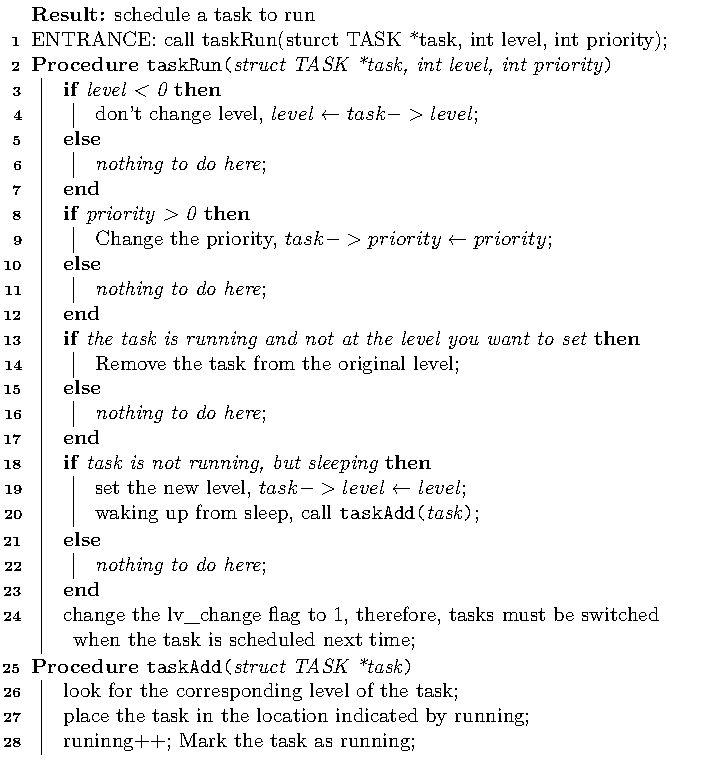
\includegraphics[width=.6\textwidth]{task-run}
  \caption{algorithm to add tasks to task pool and prepare to run}
  \label{fig:algo-add}
\end{figure}

\subsubsection{Task Scheduling and Running}
\label{sec:task-sched-runn}


The next step is for the scheduler to start scheduling task to running. The work of the
scheduler requires the support of clock interrupts. Every time a clock interrupt occurs,
the scheduler is run once. The \emph{now\_lv} variable is used to record which level is
currently running. The \emph{now} variable is a pointer to a running task of a certain
level. The specific workflow of the scheduler is described in the following steps. 


\begin{enumerate}
\item Find the currently running level \emph{tl} by \emph{now\_lv}. Move the
  \emph{now} pointer of this layer by one position. Continue to step 2.
  
\item If the number of \emph{running} tasks is equal to the \emph{now} pointer. Move back
  \emph{now} pointer to 0. Continue to step 3

\item Check if the \emph{lv\_change} flag is 1. If it is 1, check the entire \emph{task
    pool} to find the new \emph{now\_lv} and set the \emph{lv\_change} flag to 0. Continue
  to step 4.

\item Get the currently running task from \emph{now\_lv} with the \emph{now} pointer, set
  the time slice, and jump to the task to start running.
  
\end{enumerate}
Specific code implementation, see ~\ref{sec:task-scheduling} and 
~\ref{sec:task-running}. Fig. ~\ref{fig:task-schd} is the algorithm of task scheduling and
switching.
\begin{figure}[!ht]
  \centering
  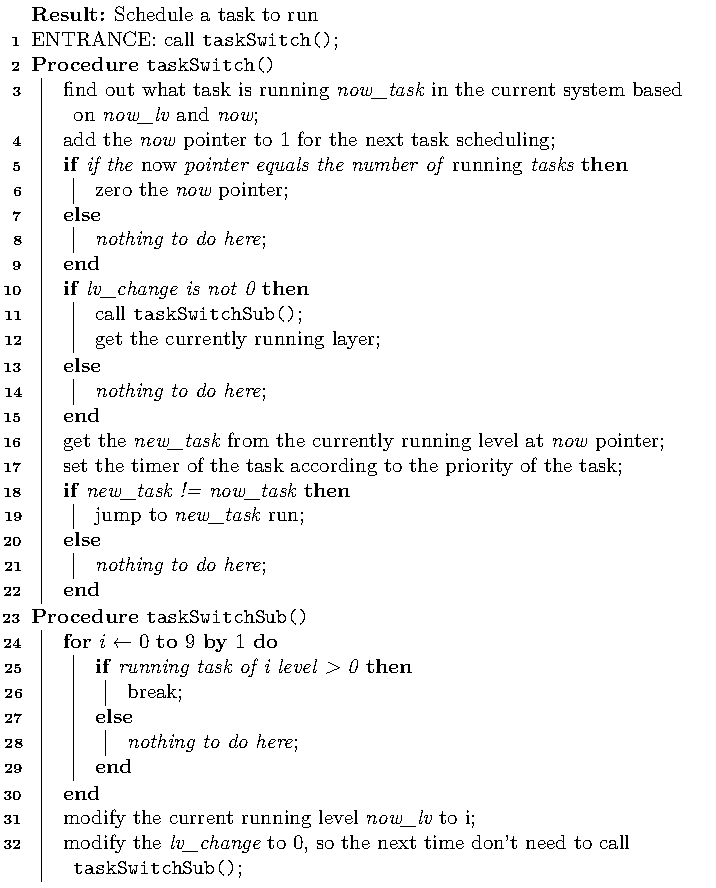
\includegraphics[width=.6\textwidth]{task-schedule} 
  \caption{task scheduling}
  \label{fig:task-schd}
\end{figure}

\subsubsection{Task Sleep}
\label{sec:task-sleep}

The task may go to \emph{sleep} after it finishes running. A task going to sleep is
actually removing it from the \emph{task pool}. Sleeping the task requires considering
whether this task is a running task. If this is the case, after the task is removed, the
task switch will be performed. Then jump to the newly switched task. These steps can be
summarized as follows
\begin{enumerate}
\item Call \emph{task\_now} to return to the currently running task. Go to the next step.
\item Call \emph{task\_remove} to remove this task from \emph{task pool}. Go to the next step.
\item The task that is going to sleep are compared with the tasks that is running. If they
  are equal, switch to the new task to start running.
  
\end{enumerate}
Specific code implementation, see ~\ref{sec:task-sleep-1}.

\subsubsection{Task\_now and Task\_remove Functions}
\label{sec:taskn-taskr-funct}
There are also two small functions that facilitate task management and are introduced
here. One is the \emph{task\_now} function and the other is the \emph{task\_remove}
function. \emph{task\_now}. The \emph{task\_now} function is used to return the address of
the task that is currently running on the system. This function is relatively simple. The
first is to find the current running level based on the \emph{now\_lv}, then the level of
the now pointer to find the task that the layer is running, and finally returns its
address.

The \emph{task\_remove} function is somewhat complicated. It may involve moving all tasks
for a layer. It may also cause various pointers to appear strange. All of these must be
considered carefully, otherwise the system may experience unpredictable and strange
behavior. Its running process can be summarized as follows.
\begin{enumerate}
\item First find the corresponding level of the task \emph{tl}. Go to the next step.
\item Find out where this task is. Go to the next step.
\item Reduce the number of processes running by 1. Go to the next step.
\item If the position of this task is before the \emph{now} pointer, the \emph{now}
  pointer is decremented by one. Go to the next step.
\item If the \emph{now} pointer is greater than the number of \emph{running} processes, it
  is necessary to correct the \emph{now} pointer to 0. Go to the next step.
\item Change the \emph{flags} of the task to 1 to indicate that the task is dormant. Go to
  the next step.
\item Move the tasks between i and \emph{running} one step forward.
  
\end{enumerate}
Specific code implementation, see ~\ref{sec:task-remove}.

\subsection{Graphic Management}
\label{sec:graphic-management}

In modern operating systems, graphics management is often not a concern of the operating
system kernel. However, as a simple multitasking 32-bit operating system with windows it
is necessary to demonstrate the implementation of a graphical management subproblem. The
issue that was selected for detailed discussion was the more complex \emph{sheet} height
settings in the graphics management section.

\subsubsection{Sheet Height Setting}
\label{sec:sheet-height-setting}

There are many \emph{sheet} on the computer screen. Which \emph{sheet} is located at which
height requires careful design and detailed consideration. When the \emph{sheet} height is set,
the height of other layers must be taken into account. When the setting is complete, the
relative height of other \emph{sheet} cannot be changed. First, the algorithm for setting
the height of the \emph{sheet} is given in Fig. ~\ref{fig:sheet-heht}.
\begin{figure}[!ht]
  \centering
  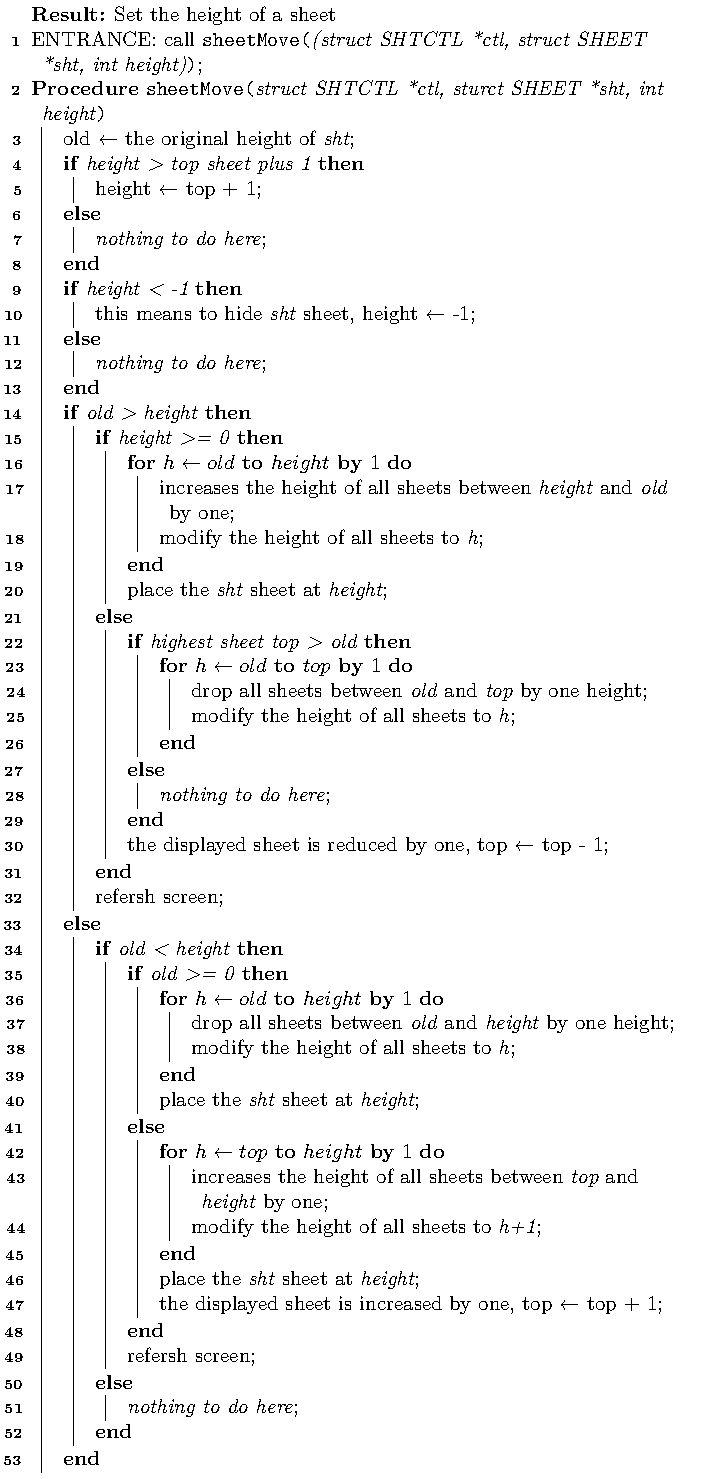
\includegraphics[width=.7\textwidth]{sheet_move_algo} 
  \caption{algorithm of sheet height setting}
  \label{fig:sheet-heht}
\end{figure}

The height of passing in may not be compliant, for example, pass a negative number and so
on. Therefore, it is necessary to check the height value first. If it does not meet the
regulations, it needs to be corrected. \emph{Sheet} height settings can be divided into
four sections.

\begin{enumerate}
\item The original height of the \emph{sheet} is higher than the newly transmitted
  height. The \emph{sheet} between the newly transmitted height and the original height
  needs to be moved upward by a height. After the move is complete, place the original
  height \emph{sheet} on the new height. Fig. ~\ref{fig:sit-one} shows this situation.
  The following explanations are necessary to understand this diagram. These explanations
  are also used for the next three cases. 1, each horizontal line represents a
  \emph{sheet}, the label on the right represents the height of the layer. 2, the old and
  new heights are mark done the left. 3, the label next to the arrow represents the order
  of movement. 4, the bottom dashed line represents the hidden \emph{sheet}, while the
  topmost dashed line represents the highest \emph{sheet}.

  \begin{figure}
    \centering
    \begin{minipage}{0.45\textwidth}
        \centering
        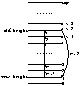
\includegraphics[width=1.2\textwidth]{sheet_move1} % first figure itself
        \caption{height setting one}
        \label{fig:sit-one}
    \end{minipage}\hfill
    \begin{minipage}{0.45\textwidth}
      \centering
      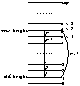
\includegraphics[width=1.2\textwidth]{sheet_move3} 
      \caption{height setting three}
      \label{fig:sit-three}
    \end{minipage}\hfill
    \begin{minipage}{0.45\textwidth}
      \centering
      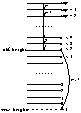
\includegraphics[width=1.2\textwidth]{sheet_move2} 
      \caption{height setting two}
      \label{fig:sit-two}
    \end{minipage}\hfill
    \begin{minipage}{0.45\textwidth}
      \centering
      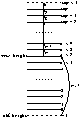
\includegraphics[width=1.2\textwidth]{sheet_move4} 
      \caption{height setting 4}
      \label{fig:sit-four}
    \end{minipage}
    \caption{all four setting height conditions}
\end{figure}
  

\item The original height of the \emph{sheet} is higher than the newly transmitted
  height. However, the height of the new pass is less than 0. This means that the
  \emph{sheet} at old height needs to be hidden, the so-called hiding is to set its height
  to -1. \emph{Sheet} above this height need to be moved down one
  height. Fig. ~\ref{fig:sit-two} shows this situation.
  

\item The original height of the \emph{sheet} is less than the newly transmitted
  height. The \emph{sheet} between the newly transmitted height and the original height
  needs to be moved down by a height. After the move is complete, place the original
  height \emph{sheet} on the new height. Fig. ~\ref{fig:sit-three} shows this situation.


\item The original height of the \emph{sheet} is less than the newly transmitted
  height. However, the height of the new pass is greater than top. This means that the
  \emph{sheet} at old height needs to be displayed, the so-called displayed is to set its height
  larger than 0. \emph{Sheet} above this new height need to be moved upward one
  height. Fig. ~\ref{fig:sit-four} shows this situation.
        
\end{enumerate}
Specific code implementation, see ~\ref{sec:graph-height-sett}.





\section{API}
\label{sec:API}


\section{APPs}
\label{sec:apps}




\chapter{Conclusions}%{Prospects And Shortages}

\footnotetext{\url{https://thesistips.wordpress.com/2012/03/25/how-to-write-your-introduction-abstract-and-summary/}}

\paragraph{What goes in your ``Conclusions'' chapter?}

{\fontspec[Scale=.8]{Purisa} The purpose of this chapter is to provide a summary of the
  whole thesis or report.  In this context, it is similar to the Abstract, except that the
  Abstract puts roughly equal weight on all thesis/report chapters, whereas the
  Conclusions chapter focuses primarily on the findings, conclusions and/or
  recommendations of the project.

  There are a couple of rules – one rigid, one common sense, for this chapter:
  \begin{itemize}
  \item All material presented in this chapter must have appeared already in the report;
    no new material can be introduced in this chapter. (rigid rule of technical writing)
  \item Usually, you would not present any new figures or tables in this chapter. (rule of thumb)
  \end{itemize}

  Generally, for most technical reports and Masters theses, the Conclusions chapter would
  be~3 to 5 pages long (double spaced).  It would generally be longer in a large PhD
  thesis. Typically you would have a paragraph or two for each chapter or major
  subsection.  Aim to include the following (typical) content.
  \begin{enumerate}
  \item Re-introduce the project and the need for the work – though more briefly than in
    the intro;
  \item Re-iterate the purpose and specific objectives of your project.
  \item Re-cap the approach taken – similar to the road map in the intro; however, in this
    case, you are re-capping the data, methodology and results as you go.
  \item Summarize the major findings and recommendations of your work.
  \item Make recommendations for future research.
  \end{enumerate}}

%%% 正文部分到此结束。下面是『参考文献』、『指导教师简介』、『鸣谢』、『附录』

%% 不要动下面四行!
\appendix{}
\maketailpages{} % 参考文献、指导教师简介、鸣谢

%%% 下面是附录部分,可以没有。

\chapter{Main Program Code} %附录一

\section{Boot loader}

\subsection{Display boot information}
\label{sec:dis-boo-inf}

\inputminted[firstline=55, lastline=65,
linenos=true]{nasm}{../../src/kernel/ipl10.asm}

\subsection{Read the second sector}
\label{sec:rea-sec-sec}
  
\inputminted[firstline=87,lastline=106,linenos=true]{nasm}{../../src/kernel/ipl10.asm}

\subsection{Read two sides of a track}
\label{sec:rea-two-sid}

\inputminted[firstline=108,lastline=132,linenos=true]{nasm}{../../src/kernel/ipl10.asm}

\subsection{The next cylinder}
\label{sec:the-nex-cyl}
\inputminted[firstline=134,lastline=137,linenos=true]{nasm}{../../src/kernel/ipl10.asm}


\section{Kernel Modules}
\label{sec:kernel-modules}
\subsection{Memory check process}
\label{sec:memory-check-process}

\inputminted[firstline=7, lastline=42, linenos=true]{c}{../../src/kernel/memory.c}
\inputminted[firstline=220, lastline=254,
linenos=true]{nasm}{../../src/kernel/naskfunc.asm}

\subsection{Memory allocation process}
\label{sec:memory-alloc-proc}
\inputminted[tabsize=2, firstline=64, lastline=85,
linenos=true]{c}{../../src/kernel/memory.c}

\subsection{Memory release process}
\label{sec:memory-rele-proc}
\inputminted[tabsize=2, firstline=88, lastline=158,
linenos=true]{c}{../../src/kernel/memory.c}

\subsection{Task allocate}
\label{sec:task-allocate}
\inputminted[tabsize=2, firstline=115, lastline=143,
linenos=true]{c}{../../src/kernel/mtask.c}


\subsection{Task add}
\label{sec:task-add}
\inputminted[tabsize=2, firstline=14, lastline=21,
linenos=true]{c}{../../src/kernel/mtask.c}

\subsection{Task scheduling}
\label{sec:task-scheduling}
\inputminted[tabsize=2, firstline=186, lastline=205,
linenos=true]{c}{../../src/kernel/mtask.c}
\inputminted[tabsize=2, firstline=49, lastline=63,
linenos=true]{c}{../../src/kernel/mtask.c}


\subsection{Task running}
\label{sec:task-running}
\inputminted[tabsize=2, firstline=146, lastline=165,
linenos=true]{c}{../../src/kernel/mtask.c}

\subsection{Task sleep}
\label{sec:task-sleep-1}
\inputminted[tabsize=2, firstline=167, lastline=184,
linenos=true]{c}{../../src/kernel/mtask.c}

\subsection{Task remove}
\label{sec:task-remove}
\inputminted[tabsize=2, firstline=23, lastline=47,
linenos=true]{c}{../../src/kernel/mtask.c}

\subsection{Graphic height setting}
\label{sec:graph-height-sett}
\inputminted[tabsize=2, firstline=250, lastline=322,
linenos=true]{c}{../../src/kernel/sheet.c}








\end{document} % 结束。不要动下面几行!

%%% Local Variables:
%%% mode: latex
%%% TeX-master: t
%%% End:
